\documentclass{article}
\usepackage[utf8]{inputenc}
\usepackage[default]{raleway}
\usepackage[table]{xcolor}
\usepackage[utf8]{inputenc}
\usepackage{pgf-pie, multirow, longtable, ragged2e, bera, subcaption, tikz, titlesec, comment, tabularx, makecell, float, listings, array, setspace, geometry, graphicx, xcolor, xparse, fancyvrb, relsize, fancyhdr, booktabs, hyperref, eurosym, todonotes}

\renewcommand{\headrulewidth}{0pt}

\colorlet{punct}{red!60!black}
\definecolor{background}{HTML}{EEEEEE}
\definecolor{delim}{RGB}{20,105,176}
\colorlet{numb}{magenta!60!black}

\lstdefinelanguage{json}{
    basicstyle=\normalfont\ttfamily,
    numbers=left,
    numberstyle=\scriptsize,
    stepnumber=1,
    numbersep=8pt,
    showstringspaces=false,
    breaklines=true,
    frame=lines,
    backgroundcolor=\color{background},
    literate=
     *{0}{{{\color{numb}0}}}{1}
      {1}{{{\color{numb}1}}}{1}
      {2}{{{\color{numb}2}}}{1}
      {3}{{{\color{numb}3}}}{1}
      {4}{{{\color{numb}4}}}{1}
      {5}{{{\color{numb}5}}}{1}
      {6}{{{\color{numb}6}}}{1}
      {7}{{{\color{numb}7}}}{1}
      {8}{{{\color{numb}8}}}{1}
      {9}{{{\color{numb}9}}}{1}
      {:}{{{\color{punct}{:}}}}{1}
      {,}{{{\color{punct}{,}}}}{1}
      {\{}{{{\color{delim}{\{}}}}{1}
      {\}}{{{\color{delim}{\}}}}}{1}
      {[}{{{\color{delim}{[}}}}{1}
      {]}{{{\color{delim}{]}}}}{1},
}

\lstdefinestyle{code}{
    frame=single,
    framesep=1mm,
    rulecolor=\color{light-gray},
    backgroundcolor=\color{light-gray},
    basicstyle=\ttfamily,
}

% ----------------------------- Definizione colori ---------------------------
\definecolor{light-gray}{gray}{0.92}
\definecolor{darkgreen}{rgb}{0.0, 0.5, 0.0}
\definecolor{navyblue}{rgb}{0.0, 0.0, 0.8}


% ----------------------------- Definizione tabella ---------------------------

\newcolumntype{C}[1]{>{\centering\arraybackslash}m{#1}}
\newcolumntype{L}[1]{>{\RaggedRight\arraybackslash}m{#1}}

% ------------------------------Metadati indice -------------------------------

\titleformat{\paragraph}[hang]{\normalfont\normalsize\bfseries}{\theparagraph}{1em}{}
\titlespacing*{\paragraph}{0pt}{0.3cm plus 0.1cm minus 0.05cm}{0.1cm plus 0.1cm minus 0.02cm}

% ------------------------------Metadati indice -------------------------------
\title{\textbf{\fontsize{30}{6}\selectfont Indice}}
\author{\fontsize{14}{6}\selectfont ByteOps}
\date{}

% -----------------------------Creazione footer --------------------------------
\pagestyle{fancy} 
\fancyhf{}
\renewcommand{\footrulewidth}{0.4pt} 
\lfoot{ 
    \parbox[c]{2cm}{
\includegraphics[width=2cm]{../Images/logo.png}}
    \textcolor[RGB]{120, 120, 120}{$\cdot$ Specifica tecnica}
}
\rfoot{\thepage}
 
% --------------------------Modifica formato hyperlinks ------------------------
\hypersetup{
    colorlinks=true,
    linkcolor=darkgreen,
    urlcolor=navyblue,
    filecolor=black,      
    pdftitle={Specifica tecnica},
    pdfpagemode=FullScreen,
}

\definecolor{responsabile}{RGB}{0,102,204}
\definecolor{amministratore}{RGB}{0,204,102}
\definecolor{analista}{RGB}{255,165,0}
\definecolor{progettista}{RGB}{255,0,0}
\definecolor{programmatore}{RGB}{128,0,128}
\definecolor{verificatore}{RGB}{255,192,203}

\definecolor{linkcolor}{rgb}{1,0,1}
\definecolor{light-gray}{gray}{0.92}
\definecolor{bgcode}{RGB}{237, 237, 237}
\definecolor{commentcolor}{RGB}{0, 153, 10}
\definecolor{bordercolor}{RGB}{56, 56, 56}

\lstset{
    language=SQL,
    basicstyle=\color{black},
    backgroundcolor=\color{bgcode},
    keywordstyle=\color{blue},
    commentstyle=\color{commentcolor},
    stringstyle=\color{red},
    numbers=left,
    numberstyle=\small,
    numbersep=-5pt,
    tabsize=4,
    showspaces=false,
    showstringspaces=false,
    breaklines=true,
    frame=single,
    rulecolor=\color{bordercolor}
}

\begin{document}
\pagestyle{fancy}
\begin{center}
    
\includegraphics[width = 0.7\textwidth]{../Images/logo.png} \\
    \vspace{0.2cm}
    \textcolor[RGB]{60, 60, 60}{\textit{ByteOps.swe@gmail.com}} \\
    \vspace{1cm}
    \fontsize{16}{6}\selectfont Specifica tecnica \\
    \vspace{0.5cm}
\end{center}

\section*{Informazioni documento}
\def\arraystretch{1.2}
\begin{tabular}{>{\raggedleft\arraybackslash}p{0.2\textwidth}|>{\raggedright\arraybackslash}p{0.6\textwidth}c}
    \hline
    \addlinespace
    \textbf{Redattori}    & A. Barutta \\ & R. Smanio \\ & L. Skenderi \\ & F. Pozza \\ & D. Diotto \\ & N. Preto \vspace{10pt} \\
    \textbf{Verificatori} & E. Hysa \\ & A. Barutta \\ & D. Diotto \\ & L. Skenderi \\ & R. Smanio \\ & F. Pozza \vspace{10pt} \\
    \textbf{Destinatari}  & ByteOps \\ & T. Vardanega \\ & R. Cardin \vspace{10pt}  \\
\end{tabular}
\pagebreak

% ------------------------- Changelog ----------------------------
\begin{tabular}{|C{1.5cm}|C{2.1cm}|C{2cm}|C{2cm}|C{4.5cm}|}
    \hline 
    \textbf{Versione} & \textbf{Data} & \textbf{Autore} & \textbf{Verificatore} & \textbf{Dettaglio} \\
    \hline
    \label{Git_Action_Version} 0.4.0 & 18/03/2024 & F. Pozza & L. Skenderi & Conclusione sezione Tabella dei requisiti soddisfatti \\ 
    \hline
    0.3.1 & 15/03/2024 & E. Hysa & A. Barutta & Iniziale stesura sezione Tabella dei requisiti soddisfatti \\ 
    \hline
    0.3.0 & 12/03/2024 & N. Preto & D. Diotto & Conclusione sezione Architettura di deployment \\ 
    \hline
    0.2.1 & 08/03/2024 & R. Smanio & A. Barutta & Iniziale stesura sezione Architettura di deployment \\  
    \hline
    0.2.0 & 07/03/2024 & E. Hysa & A. Barutta & Completamento scrittura sottosezione 3.7, correzioni ulteriori sezione Architettura di sistema \\ 
    \hline
    0.1.5 & 05/03/2024 & N. Preto & R. Smanio & Completamento scrittura sottosezione 3.5 e 3.6 \\ 
    \hline
    0.1.4 & 04/03/2024 & N. Preto & R. Smanio & Completamento scrittura sottosezione 3.4 \\ 
    \hline
    0.1.3 & 01/03/2024 & F. Pozza & A. Barutta & Completamento scrittura sottosezione 3.3  \\ 
    \hline
    0.1.2 & 24/02/2024 & F. Pozza & E. Hysa & Completamento scrittura sottosezioni 3.1 e 3.2 \\ 
    \hline
    0.1.1 & 22/02/2024 & D. Diotto & R. Smanio & Iniziale stesura sezione Architettura di sistema \\ 
    \hline
    0.1.0 & 16/02/2024 & E. Hysa & R. Smanio & Conclusione sezione Tecnologie \\
    \hline
    0.0.2 & 08/02/2024 & A. Barutta & F. Pozza & Continuazione stesura Tecnologie \\
    \hline
    0.0.2 & 05/02/2024 & A. Barutta & F. Pozza & Stesura sezione Introduzione, inizio stesura sezione Tecnologie \\ 
    \hline
    0.0.1 & 01/02/2024 & E. Hysa & A. Barutta & Impostazione sezioni \\ 
    \hline 
\end{tabular}

\pagebreak

% ------------------------- Generazione automatica indice ----------------------
\setstretch{1.5}
\maketitle
\thispagestyle{fancy}
{
    \hypersetup{linkcolor=black}
    \tableofcontents
    \setcounter{tocdepth}{4}
    \listoffigures
}
\setstretch{1.2}
\pagebreak

% ---------------------------- Inizio documento -------------------------------

\flushleft

\section{Introduzione}

\subsection{Scopo del Manuale}
Il manuale ha lo scopo di assistere l’utente passo dopo passo per un corretto utilizzo del
software così da sfruttarne appieno tutte le funzionalità presenti per offrire un’esperienza
ottimale

\subsection{Glossario}
Incluso nella documentazione è presente il \textbf{\textit{Glossario}} in cui sono definiti tutti i termini specifici o eventualmente ambigui presenti nei vari documenti del progetto. Se un termine è nel \textbf{\textit{Glossario}}, viene segnalato con una \textit{G} a pedice accanto ad esso.

\subsubsection{Raccolta termini del glossario}
Il \textbf{\textit{Glossario}} verrà compilato attraverso un documento condiviso su \LaTeX \textsubscript{\textit{G}}, accessibile a ttti i membri del gruppo. Qui, verranno elencati i ter min  i di particolare rilevanza nel contesto del progetto, seguendo una checklist.   Successivamente, l'\textit{Amministratore} del progetto si occuperà di dettagliare  ulteriormente questi termini nella creazione del \textbf{\textit{Glossario}} ufficiale. 
\subsection{Riferimenti}
\subsubsection{Riferimenti informativi}
    \begin{itemize}
        \item \href {https://www.math.unipd.it/~tullio/IS-1/2023/Progetto/C6.pdf} {Capitolato d'appalto C6 - InnovaCity }
        \item \href{https://www.math.unipd.it/~tullio/IS-1/2023/Dispense/T4.pdf} {Slide del corso di Ingegneria del Software - Gestione di progetto }
        \item \href{https://www.math.unipd.it/~tullio/IS-1/2023/Dispense/T2.pdf} {Slide del corso di Ingegneria del Software - Ciclo di vita del software }
    \end{itemize}
 
\subsubsection{Riferimenti normativi}
    \begin{itemize}
    \item Norme di progetto
    \item \href {https://www.math.unipd.it/~tullio/IS-1/2023/Dispense/PD2.pdf} {Regolamento del progetto didattico }
    \end{itemize}

\vspace{0.5cm}

\section{Tecnologie}
In questa sezione sono definiti gli strumenti e le tecnologie impiegati per lo sviluppo e l'implementazione del software relativo al progetto InnovaCity.

Si procederà quindi con la descrizione delle tecnologie e dei linguaggi di programmazione utilizzati, delle librerie e dei framework necessari, nonché delle infrastrutture richieste.

L'obiettivo principale è garantire che il software sia sviluppato utilizzando le tecnologie più appropriate e selezionando le opzioni ottimali in termini di efficienza, sicurezza e affidabilità.

\subsection{Docker}
Per lo sviluppo, il testing e il rilascio del prodotto sono stati utilizzati container Docker in modo tale da garantire ambienti consistenti e riproducibili.

\subsubsection{Ambienti}
\begin{itemize}
  \item \textbf{Ambiente di sviluppo:}
    \begin{itemize}
      \item È l'ambiente dove i software developer scrivono, testano e modificano il codice sorgente;
      \item Può includere strumenti di debug e monitoraggio per facilitare lo sviluppo e la correzione di errori;
      \item Non è accessibile agli utenti finali.
    \end{itemize}
    \item \textbf{Ambiente di test:}
    \begin{itemize}
      \item Simula l'ambiente di produzione;
      \item Viene utilizzato per testare il software in modo completo e realistico prima del rilascio in produzione;
      \item I test possono essere automatizzati o manuali e includono test di unità, integrazione, sicurezza e prestazioni.
    \end{itemize}
    \item \textbf{Ambiente di produzione:}
    \begin{itemize}
      \item È l'ambiente dove il software viene rilasciato per poter essere utilizzato dagli utenti finali;
      \item Deve essere stabile, sicuro e performante per garantire un'esperienza utente ottimale;
      \item Le modifiche al software in produzione sono controllate rigorosamente per minimizzare i rischi di errori o downtime.
    \end{itemize}
\end{itemize}

\subsubsection{Docker images}

Di seguito sono elencate le immagini Docker utilizzate:

\begin{itemize}

  \item \textbf{Simulators - Python} 
    \begin{itemize}
      \item \textbf{Image:} Python:3.9;
      \item \textbf{Riferimento:} \url{https://hub.docker.com/_/python}~(consultato: 19/03/2024);
      \item \textbf{Ambiente:}
        \begin{itemize}
          \item Develop;
          \item Production.
        \end{itemize}
    \end{itemize}

  \item \textbf{Broker - Apache Kafka} 
    \begin{itemize}
      \item \textbf{Image:} bitnami/kafka:latest;
      \item \textbf{Riferimento:} \url{https://hub.docker.com/layers/bitnami/kafka/latest/images/sha256-4894d89d28f8e06a7d8a064efdc2dc9cb61dd205721c61296b6d033ad4824a91?context=explore}~(consultato: 19/03/2024);
      \item \textbf{Ambiente:}
        \begin{itemize}
          \item Develop;
          \item Production;
          \item Testing;
        \end{itemize}
    \end{itemize}

  \item \textbf{Apache Kafka UI} 
    \begin{itemize}
      \item \textbf{Image:}
      \item \textbf{Riferimento:}
      \item \textbf{Ambiente:}
        \begin{itemize}
          \item Develop.
        \end{itemize}
    \end{itemize}

  \item \textbf{Schema registry} 
    \begin{itemize}
      \item \textbf{Image:}
      \item \textbf{Riferimento:}
      \item \textbf{Ambiente:}
        \begin{itemize}
          \item Develop;
          \item Production;
          \item Testing;
        \end{itemize}
    \end{itemize}

  \item \textbf{Schema registry UI} 
    \begin{itemize}
      \item \textbf{Image:}
      \item \textbf{Riferimento:}
      \item \textbf{Ambiente:}
        \begin{itemize}
          \item Develop.
        \end{itemize}
    \end{itemize}

  \item \textbf{Faust processing - Python} 
    \begin{itemize}
      \item \textbf{Image:}
      \item \textbf{Riferimento:}
      \item \textbf{Ambiente:}
        \begin{itemize}
          \item Develop;
          \item Production;
          \item Testing;
        \end{itemize}
    \end{itemize}

  \item \textbf{ClickHouse} 
    \begin{itemize}
      \item \textbf{Image:}
      \item \textbf{Riferimento:}
      \item \textbf{Ambiente:}
        \begin{itemize}
          \item Develop;
          \item Production;
          \item Testing;
        \end{itemize}
    \end{itemize}

  \item \textbf{Grafana} 
    \begin{itemize}
      \item \textbf{Image:}
      \item \textbf{Riferimento:}
      \item \textbf{Ambiente:}
        \begin{itemize}
          \item Develop;
          \item Production.
        \end{itemize}
    \end{itemize}
\end{itemize}

\subsection{Linguaggi e formato dati}
\subsubsection{Python}
Linguaggio di programmazione ad alto livello, interpretato e multi-paradigma.

\paragraph{Versione:}
Versione utilizzata: 3.9
\paragraph{Documentazione:}
\url{https://docs.python.org/release/3.9.0/}

\paragraph{Utilizzo nel progetto} 
\begin{itemize}
    \item Creazione delle simulazioni dei sensori, incluse le logiche di scrittura e invio dei dati registrati;
    \item Modello per il calcolo del punteggio di salute della città;
    \item Testing.
\end{itemize}

\paragraph{Librerie o framework}

\begin{itemize}
    \item \textbf{Confluent Kafka}
    \begin{itemize}
        \item \textbf{Documentazione:} \url{https://developer.confluent.io/get-started/python/}~(consultato: 19/03/2024);
        \item \textbf{Versione:} 2.3.0;
        \item Libreria Python che fornisce un insieme completo di strumenti per agevolare la produzione e il consumo di messaggi da Apache Kafka.
    \end{itemize}
    
    \item \textbf{Faust}
    \begin{itemize}
        \item \textbf{Documentazione:} \url{https://faust.readthedocs.io/en/latest/}~(consultato: 19/03/2024);
        \item \textbf{Versione:} 1.10.4;
        \item Framework Python per la creazione di applicazioni di data streaming in tempo reale. Fornisce un'API dichiarativa e funzionale per definire i flussi di dati e le trasformazioni, consentendo agli sviluppatori di scrivere facilmente applicazioni scalabili e affidabili per il trattamento di grandi volumi di dati in tempo reale.
        
        Faust si integra nativamente con Apache Kafka e offre funzionalità avanzate come il bilanciamento del carico, la gestione dello stato, la gestione delle query, e la tolleranza ai guasti, rendendolo una scelta ottimale per lo sviluppo di sistemi di data streaming complessi e robusti.
    \end{itemize}
    
    \item \textbf{Pytest}
    \begin{itemize}
        \item \textbf{Documentazione:} \url{https://docs.pytest.org/en/7.1.x/contents.html}~(consultato: 19/03/2024);
        \item \textbf{Versione:} 8.0.2;
        \item Framework di testing per Python, noto per la sua semplicità. Consente agli sviluppatori di scrivere test chiari e concisi utilizzando una sintassi intuitiva e flessibile.
        
        Pytest supporta una vasta gamma di funzionalità, tra cui test di unità, integrazione e accettazione, parametrizzazione dei test e gestione delle fixture.

        Merita menzione anche l'utilizzo di \textit{Pytest-asyncio} per testare codice asincrono e \textit{Pytest-cov} per la copertura del codice.
    \end{itemize}
    
    \item \textbf{Pylint}
    \begin{itemize}
        \item \textbf{Documentazione:} \url{https://pylint.readthedocs.io/en/stable/}~(consultato: 19/03/2024);
        \item \textbf{Versione:} 3.1.0;
        \item Strumento di analisi statica per il linguaggio di programmazione Python. Esamina il codice sorgente per individuare potenziali errori, conformità alle linee guida stilistiche e altre possibili fonti di bug nel codice Python. Inoltre, valuta anche la qualità del codice in termini di \textit{good practice} di programmazione.
        
        Pylint fornisce un punteggio di qualità del codice e suggerimenti per migliorare la leggibilità, la manutenibilità, sicurezza e la correttezza del codice Python.
    \end{itemize}
    
    \item \textbf{Clickhouse-connect}
    \begin{itemize}
        \item \textbf{Documentazione:} \url{https://clickhouse.com/docs/en/integrations/python}~(consultato: 19/03/2024);
        \item \textbf{Versione:} 0.7.2;
        \item ClickHouse Connect è una libreria open source sviluppata per semplificare l'interazione con il database ClickHouse tramite il linguaggio di programmazione Python, viene utilizzata nei test.
        
        Essa fornisce un'interfaccia per comunicare con ClickHouse, consentendo agli sviluppatori di eseguire query, inserire dati e gestire altri aspetti dell'interazione con il database in modo efficiente e conveniente.
    \end{itemize}
\end{itemize}

\subsubsection{SQL (Structured Query Language)}
Linguaggio standard per la gestione e la manipolazione dei
database che lo supportano. \todo{arricchire un po' questa parte}

\paragraph{Utilizzo nel progetto}
Gestione e interrogazione database Clickhouse.


\subsection{JSON (JavaScript Object Notation)}
JSON è un formato di scrittura leggibile dalle persone e facilmente interpretabile dai computer. È utilizzato principalmente per lo scambio di dati strutturati attraverso le reti, come Internet.

Il formato JSON si basa su due strutture di dati principali:

\begin{itemize}
  \item \textbf{Oggetti}: Rappresentati da coppie chiave-valore racchiuse tra parentesi graffe \{ \}, dove la chiave è una stringa e il valore può essere un altro oggetto, un array, una stringa, un numero, un booleano o \texttt{null}.
  \item \textbf{Array}: Una raccolta ordinata di valori, racchiusi tra parentesi quadre [ ], in cui ogni elemento può essere un oggetto, un array, una stringa, un numero, un booleano o \texttt{null}.
\end{itemize}

JSON offre una sintassi semplice e chiara per la rappresentazione dei dati, che lo rende ampiamente utilizzato in molti contesti, inclusi lo sviluppo web, le API di servizi web e lo scambio di dati tra applicazioni. La sua leggibilità e la sua natura basata su testo lo rendono particolarmente adatto per l'interazione tra sistemi eterogenei.

Nel nostro contesto viene utilizzato per scambiare i dati dai simulatori \textit{Python} a \textit{kafka}, e dal server \textit{kafka} a \textit{Clickhouse}.
\subsubsection{YAML (YAML Ain't Markup Language)}
Formato di serializzazione leggibile dall'uomo utilizzato per rappresentare dati strutturati in modo chiaro e semplice.

\paragraph{Utilizzo nel progetto}
\begin{itemize}
    \item Configurazione
    docker compose;
    \item Configurazione pipeline Git-Hub workflow per Countinuous Integration;
    \item Configurazione provisioning Grafana e politiche di notifica allerte.
\end{itemize}

\subsection{Database e servizi}
\subsubsection{Apache Kafka}
Apache Kafka è una piattaforma open-source di streaming distribuito sviluppata dall'Apache Software Foundation. Progettata per gestire flussi di dati in tempo reale in modo scalabile e affidabile, è ampiamente utilizzata nel data streaming e nell'integrazione dei dati nelle moderne applicazioni.

\paragraph{Versione}
La versione utilizzata è: 3.7.0
\paragraph{Documentazione}
\href{https://kafka.apache.org/20/documentation.html}{https://kafka.apache.org/20/documentation.html}

\paragraph{Funzionalità e vantaggi di Apache Kafka}
Le principali funzionalità e vantaggi di Apache Kafka includono:

\begin{itemize}
  \item \textbf{Pub-Sub Messaging:} Kafka utilizza un modello di messaggistica publish-subscribe, dove i produttori di dati inviano messaggi ad uno o più topic e i consumatori possono sottoscriversi a tali topic per ricevere i messaggi;
  
  \item \textbf{Disaccoppiamento Produttore - Consumatore:} questo principio si realizza grazie al fatto che i Produttori e i Consumatori non necessitano di essere consapevoli l'uno dell'altro o di interagire direttamente. Invece, essi comunicano attraverso il broker Kafka, che svolge il ruolo di intermediario per la trasmissione dei messaggi. Ciò consente una maggiore scalabilità e flessibilità nell'architettura del sistema, facilitando la gestione e il mantenimento delle applicazioni;
  
  \item \textbf{Architettura Distribuita:} Kafka è progettato per essere distribuito su un cluster di nodi, consentendo una scalabilità orizzontale per gestire grandi volumi di dati e carichi di lavoro. Questo approccio distribuito offre resilienza e alta disponibilità, garantendo che il sistema possa crescere in modo flessibile con l'aumentare delle richieste;
  
  \item \textbf{Persistenza e Affidabilità:} Kafka offre la possibilità di definire politiche specifiche per la conservazione dei dati, garantendo la durabilità dei messaggi. Questo non solo assicura la disponibilità dei dati anche in caso di eventuali interruzioni del servizio, ma consente anche ai consumatori di recuperare i messaggi dopo tali anomalie, garantendo un alto livello di affidabilità nel sistema.
  
  \item \textbf{Alta Disponibilità:} Kafka assicura un'elevata disponibilità e tolleranza ai guasti grazie alla sua architettura distribuita e al meccanismo di replica dei dati. Anche in caso di malfunzionamenti dei nodi o delle componenti, i cluster di Kafka mantengono la loro operatività, garantendo la continuità del servizio.
  
  \item \textbf{Elaborazione degli Stream:} Kafka supporta anche l'elaborazione degli stream di dati in tempo reale tramite API come Kafka Streams e Kafka Connect, consentendo agli sviluppatori di scrivere applicazioni per l'analisi e l'elaborazione dei dati in tempo reale.
\end{itemize}

\paragraph{Casi d'uso di Apache Kafka}

Apache Kafka è utilizzato in una vasta gamma di casi d'uso, tra cui:

\begin{itemize}
  \item \textbf{Data Integration:} Kafka viene utilizzato per integrare dati provenienti da diverse fonti e sistemi, consentendo lo scambio di dati in tempo reale tra applicazioni e sistemi eterogenei.
  
  \item \textbf{Streaming di Eventi:} Molte applicazioni moderne, come le applicazioni IoT (Internet of Things) e le applicazioni di monitoraggio in tempo reale, utilizzano Kafka per lo streaming di eventi in tempo reale e l'analisi dei dati.
  
  \item \textbf{Analisi dei Log:} Kafka è spesso utilizzato per l'analisi dei log di sistema e applicativi in tempo reale, consentendo il monitoraggio delle prestazioni, la rilevazione degli errori e l'analisi dei pattern di utilizzo.
  
  \item \textbf{Elaborazione di Big Data:} Kafka è integrato con tecnologie di big data come Apache Hadoop e Apache Spark, consentendo l'elaborazione di grandi volumi di dati in tempo reale.
  
  \item \textbf{Messaggistica Real-time:} Kafka è ampiamente utilizzato per la messaggistica real-time in applicazioni di social media, e-commerce e finanziarie, dove la velocità e l'affidabilità della messaggistica sono cruciali.
\end{itemize}

\paragraph{Utilizzo nel progetto}
\textit{Kafka} funge da intermediario dei messaggi, ricevendo i dati dai produttori e rendendoli disponibili ai consumatori. Nel contesto del progetto, i dati provenienti dalle simulazioni di sensori vengono inviati a \textit{Kafka} come messaggi in formato \textit{JSON}.

\paragraph*{Consumatori di dati:}
\begin{itemize}
  \item \textbf{\textit{ClickHouse:}} \textit{Kafka} invia \todo{è Kafka che li invia o i consumatori che se li prendono da Kafka?} i dati ai consumatori, inclusi i database come \textit{ClickHouse}, dove i dati vengono salvati per l'analisi e l'archiviazione a lungo termine.
  \item \textbf{\textit{Faust:}} per soddisfare il requisito opzionale del calcolo del punteggio di salute, \textit{Kafka} rende disponibili i dati in tempo reale a un'applicazione di Faust\todo{è corretto applicazione di Faust?}. Quest'ultima elabora i dati utilizzando una funzione di aggregazione per calcolare il punteggio e quindi mette a disposizione il risultato in una coda dedicata di Kafka per i servizi interessati.
\end{itemize}

In breve, \textit{Kafka} funge da ponte tra i produttori di dati (simulazioni di sensori) e i consumatori di dati (\textit{ClickHouse} o altri servizi futuri). Gestisce il flusso dei dati in tempo reale e garantisce che i dati siano disponibili per l'elaborazione e la visualizzazione in modo efficiente e scalabile.
\subsubsection{Schema Registry}
Schema Registry è un componente importante nell'ecosistema di Apache Kafka, progettato per la gestione e la convalida degli schemi dei dati utilizzati all'interno di un sistema di messaggistica distribuita.

\paragraph{Funzionalità e Vantaggi di Schema Registry}
Le funzionalità principali di Schema Registry includono:
\begin{itemize}
    \item \textbf{Gestione centralizzata degli schemi}: Fornisce un repository centralizzato per la gestione degli schemi dei dati.
    \item \textbf{Convalida degli schemi}: Assicura la validità e la compatibilità degli schemi dei dati.
    \item \textbf{Serializzazione e deserializzazione}: Supporta la serializzazione e la deserializzazione dei dati basati sugli schemi su reti distribuite.
    \item \textbf{Governance dei dati}: Contribuisce alla governance dei dati garantendo la qualità, la conformità agli standard e la tracciabilità dei dati.
\end{itemize}

\paragraph{Casi d'uso di Schema Registry}

Schema Registry è utilizzato in una vasta gamma di casi d'uso, tra cui:

\begin{itemize}
\item \textbf{Garanzia della compatibilità dei dati:} Schema Registry garantisce la compatibilità dei dati tra produttori e consumatori, consentendo l'evoluzione degli schemi dei dati senza interruzioni nei flussi di lavoro.

\item \textbf{Gestione della versione degli schemi:} Fornisce un sistema per gestire diverse versioni degli schemi dei dati, permettendo agli sviluppatori di aggiornare gli schemi in modo controllato e gestire la migrazione dei dati tra le versioni.

\item \textbf{Conformità agli standard e governance dei dati:} Aiuta a garantire la conformità agli standard aziendali e normativi, fornendo strumenti per la convalida degli schemi e la tracciabilità delle modifiche nel tempo.

\item \textbf{Collaborazione tra team e integrazione dei sistemi:} Funge da punto centrale per la collaborazione tra team di sviluppo, consentendo loro di condividere, discutere e approvare gli schemi dei dati per un'integrazione più efficace dei sistemi.

\item \textbf{Controllo della qualità dei dati:} Schema Registry contribuisce a garantire la qualità dei dati, riducendo il rischio di errori dovuti a incompatibilità o a dati non validi all'interno del sistema.
\end{itemize}


\paragraph{Utilizzo nel progetto}
Nell'ambito del progetto didattico Schema registry permette di validare i messaggi nell'ambito del topic kakfa di appartenenza definendo un contratto che i produttori, ovvero i sensori, dovranno rispettare nell'invio delle misurazioni.
\subsubsection{Zookeper}
Apache ZooKeeper è un servizio di coordinamento open-source sviluppato dalla Apache Software Foundation. È progettato per fornire funzionalità di coordinazione affidabili e scalabili per applicazioni distribuite.

\paragraph*{Versione:}


\paragraph*{Documentazione:}
\href{https://zookeeper.apache.org/documentation.html}{https://zookeeper.apache.org/documentation.html}
\paragraph*{Funzionalità e vantaggi di Apache ZooKeeper:}
Le principali funzionalità e vantaggi di Apache ZooKeeper includono:
\begin{itemize}
    \item \textbf{Servizio di coordinazione centralizzato:}ZooKeeper fornisce un servizio centralizzato per la gestione delle configurazioni, l'elezione del leader, la sincronizzazione dei dati e la notifica di eventi.
    \item \textbf{Affidabilità e scalabilità:} ZooKeeper è progettato per essere affidabile e scalabile, in grado di gestire grandi cluster di applicazioni distribuite.
    \item \textbf{Integrazione con altri software:} ZooKeeper è integrato con molti altri software open-source, tra cui Apache Kafka, Apache Hadoop e Apache HBase.
\end{itemize}
 
\paragraph*{Casi d'uso di Apache ZooKeeper:}

Apache ZooKeeper è utilizzato in una vasta gamma di casi d'uso, tra cui:
\begin{itemize}
    \item Naming service;
    \item Configuration management;
    \item Data Synchronization;
    \item Leader election;
    \item Message queue;
    \item Notification system.
\end{itemize}

\paragraph*{Utilizzo nel progetto:}
ZooKeeper è utilizzato principalmente:
\begin{itemize}
    \item \textbf{Sincronizzazione dei nodi Kafka}: Memorizza la configurazione del cluster Kafka, inclusa la lista dei broker attivi.
    Quando un nuovo broker viene aggiunto, ZooKeeper aggiorna la configurazione e notifica gli altri broker.
    Questo garantisce che tutti i broker abbiano una visione coerente del cluster e possano comunicare correttamente.
    \item \textbf{Coordinamento dello Schema Registry}:Memorizza lo schema per tutti i topic Kafka utilizzati nel progetto.
    Quando un client tenta di produrre un messaggio su un topic, lo Schema Registry verifica lo schema con ZooKeeper.
    Se lo schema è compatibile, il messaggio viene accettato. In caso contrario, il messaggio viene rifiutato.
    Questo garantisce che solo messaggi con schemi validi vengano pubblicati sui topic.
    
\end{itemize}

\subsection{ClickHouse} \label{sec:clickHouse}
ClickHouse è un sistema di gestione di database (DBMS) di tipo column-oriented, progettato principalmente per l'analisi di grandi volumi di dati in tempo reale. È un progetto open-source sviluppato da Yandex, un motore di ricerca russo, ed è stato creato per rispondere alle esigenze di elaborazione analitica ad alte prestazioni.
\subsubsection{Versione}
La versione utilizzata è: 24.1.5.6
\subsubsection{Link download}
\href{https://clickhouse.com/}{https://clickhouse.com/}

\subsubsection*{Funzionalità e Vantaggi di ClickHouse}
\begin{itemize}
    \item \textbf{ Modello di dati column-oriented:} a differenza dei tradizionali DBMS che memorizzano i dati in modo row-oriented, dove le righe complete sono memorizzate in sequenza, ClickHouse memorizza i dati in modo column-oriented. Questo significa che i dati di ogni colonna sono memorizzati insieme, permettendo una maggiore compressione e velocità di query per le analisi che coinvolgono molte colonne;
    \item \textbf{Architettura Distribuita e scalabilità:} ClickHouse è progettato per funzionare in un ambiente distribuito, consentendo la scalabilità orizzontale per gestire grandi carichi di lavoro;
    \item \textbf{Compressione dei Dati:} utilizza algoritmi efficienti per ridurre lo spazio di archiviazione richiesto per i dati, riducendo i costi di archiviazione;
    \item \textbf{Alte Prestazioni:} ottimizzato per eseguire query analitiche su grandi volumi di dati in tempo reale, garantendo tempi di risposta bassi anche con carichi di lavoro elevati.
    \item \textbf{Supporto per SQL:} supporta un sottoinsieme del linguaggio SQL, consentendo agli sviluppatori di scrivere query complesse per l'analisi dei dati;
    \item \textbf{Integrazione con Strumenti di Business Intelligence (BI):} può essere integrato con strumenti di BI popolari come Tableau, Power BI, Qlik, Grafana per la visualizzazione e l'analisi dei dati.
\end{itemize}


\subsubsection*{Casi d'Uso di ClickHouse}
ClickHouse è adatto per una vasta gamma di casi d'uso, tra cui:
\begin{itemize}
    \item \textbf{Analisi dei Log:} clickHouse può essere utilizzato per analizzare i log di grandi dimensioni generati da server, applicazioni web e dispositivi IoT;
    \item \textbf{Analisi dei Dati in Tempo Reale:} ClickHouse è ideale per l'analisi dei dati in tempo reale, consentendo agli utenti di eseguire query complesse su flussi di dati in continua evoluzione;
    \item \textbf{Reporting e Dashboard:} ClickHouse può essere utilizzato per generare report e dashboard interattivi per monitorare le prestazioni del business e identificare tendenze.
\end{itemize}



\subsection{Grafana}
Grafana è una piattaforma open-source per la visualizzazione e l'analisi dei dati, utilizzata per creare dashboard interattive e grafici da fonti di dati eterogenee. 
\subsubsection{Versione}
La versione utilizzata è: x.x.x
\subsubsection{Link download}
\href{https://clickhouse.com/}{https://clickhouse.com/}

\subsubsection{Funzionalità e Vantaggi di Grafana}
\begin{itemize}
    \item \textbf{Dashboard interattive}: Creazione di dashboard personalizzate e interattive per visualizzare dati provenienti da diverse fonti in un'unica interfaccia.
    
    \item \textbf{Connessione a sorgenti di dati eterogenee}: Supporto per una vasta gamma di sorgenti di dati, inclusi database, servizi cloud, sistemi di monitoraggio, API e altro ancora.
    
    \item \textbf{Ampia varietà di visualizzazioni}: Selezione di pannelli e visualizzazioni, tra cui grafici a linea, a barre, a torta, termometri, mappe geografiche e altro ancora, per adattarsi alle esigenze specifiche di visualizzazione dei dati.
    
    \item \textbf{Query e aggregazioni flessibili}: Esecuzione di query flessibili e aggregazione dei dati in modi personalizzati per ottenere insight approfonditi dai dati.
    
    \item \textbf{Notifiche e allarmi}: Impostazione di avvisi in base a criteri predefiniti, come soglie di performance, e ricezione di notifiche tramite diversi canali, tra cui email, Slack e molti altri.
    
    \item \textbf{Gestione degli accessi e dei permessi}: Controllo degli accessi e dei permessi degli utenti in modo granulare, gestendo chi può visualizzare, modificare o creare dashboard e pannelli.
    
    \item \textbf{Integrazione con altre applicazioni e strumenti}: Integrazione con una vasta gamma di applicazioni e strumenti, tra cui sistemi di log management, strumenti di monitoraggio delle prestazioni, sistemi di allerta e altro ancora.
    
   \end{itemize}
\subsubsection{Casi d'Uso di Grafana}
\begin{itemize}
    \item \textbf{Monitoraggio delle prestazioni}: Monitoraggio in tempo reale delle metriche di sistema come CPU, memoria e rete per identificare e risolvere rapidamente problemi di prestazioni.
    
    \item \textbf{Analisi dei log}: Analisi e visualizzazione dei log delle applicazioni e dell'infrastruttura per individuare pattern e risolvere problemi operativi.
    
    \item \textbf{Monitoraggio dell'infrastruttura}: Monitoraggio dello stato e delle prestazioni di server, servizi cloud, database e altri componenti IT per garantire un funzionamento ottimale dell'infrastruttura.
    
    \item \textbf{DevOps e CI/CD}: Monitoraggio dei processi di sviluppo, test e distribuzione del software per migliorare la collaborazione e l'efficienza del team.
    
    \item \textbf{Monitoraggio di dispositivi IoT}: Monitoraggio dei dispositivi IoT per raccogliere e visualizzare dati di sensori e dispositivi connessi, consentendo una gestione efficiente degli ambienti IoT.
\end{itemize}
\subsubsection{Utilizzo nel progetto}
Nel contesto di un progetto che coinvolge la visualizzazione e l'analisi di miliardi di misurazioni di sensori IoT, Grafana viene utilizzato principalmente per:

\begin{itemize}
  \item \textbf{Visualizzazione dei dati}: Grafana consente agli utenti di creare dashboard personalizzate e grafici interattivi che mostrano i dati provenienti dai sensori IoT in modo chiaro e comprensibile. Questi grafici possono essere configurati per visualizzare metriche specifiche nel formato desiderato, consentendo agli utenti di monitorare facilmente le prestazioni dei sensori e rilevare eventuali pattern o anomalie nei dati.
  
  \item \textbf{Analisi dei dati}: Grafana offre una vasta gamma di opzioni per analizzare i dati, inclusi filtri, aggregazioni, calcoli e altro ancora. Gli utenti possono eseguire query sui dati direttamente da Grafana e visualizzare i risultati in grafici, permettendo loro di ottenere una comprensione più approfondita delle tendenze e dei modelli presenti nei dati dei sensori IoT.
  
  \item \textbf{Monitoraggio in tempo reale}: Grafana supporta il monitoraggio in tempo reale dei dati, consentendo agli utenti di visualizzare aggiornamenti istantanei sui valori dei sensori e le metriche correlate. Ciò è particolarmente utile per l'analisi delle prestazioni in tempo reale e per la rilevazione immediata di problemi o anomalie nei dati dei sensori.
  
  \item \textbf{Allerta e notifica}: Grafana offre funzionalità avanzate di allerta e notifica che consentono agli utenti di impostare avvisi basati su condizioni specifiche dei dati. Ad esempio, è possibile configurare Grafana per inviare notifiche via email o tramite servizi di messaggistica istantanea quando un determinato sensore supera una soglia prestabilita o quando si verifica un'anomalia nei dati.
\end{itemize} 



\section{Architettura}

Il sistema richiede la capacità di elaborare dati provenienti da diverse fonti in tempo reale e di fornire una visualizzazione immediata e continua di tali dati, permettendo di monitorarne gli andamenti e di rilevare eventuali anomalie. 
Per tale scopo, l'architettura di sistema adottata è la \textit{$\kappa$-architecture}.

\subsubsection{$\kappa$-architecture}
L'architettura Kappa è un modello di elaborazione dati in streaming che offre un'alternativa all'architettura Lambda. Il suo obiettivo principale è unificare l'elaborazione in tempo reale e batch (per i dati storici) all'interno di un unico stack tecnologico.
\paragraph{Vantaggi}
\begin{itemize}
    \item Semplice da implementare e gestire, costi di manutenzione ridotti;
    \item Assicura coerenza tra l'analisi in tempo reale e batch.
\end{itemize}
\paragraph*{Svantaggi}
\begin{itemize}
    \item Potenziale rallentamento dell'analisi in tempo reale, meno flessibile rispetto a Lambda.
\end{itemize}

\subsubsection{Componenti di sistema}
\begin{figure}[H]
    \centering
    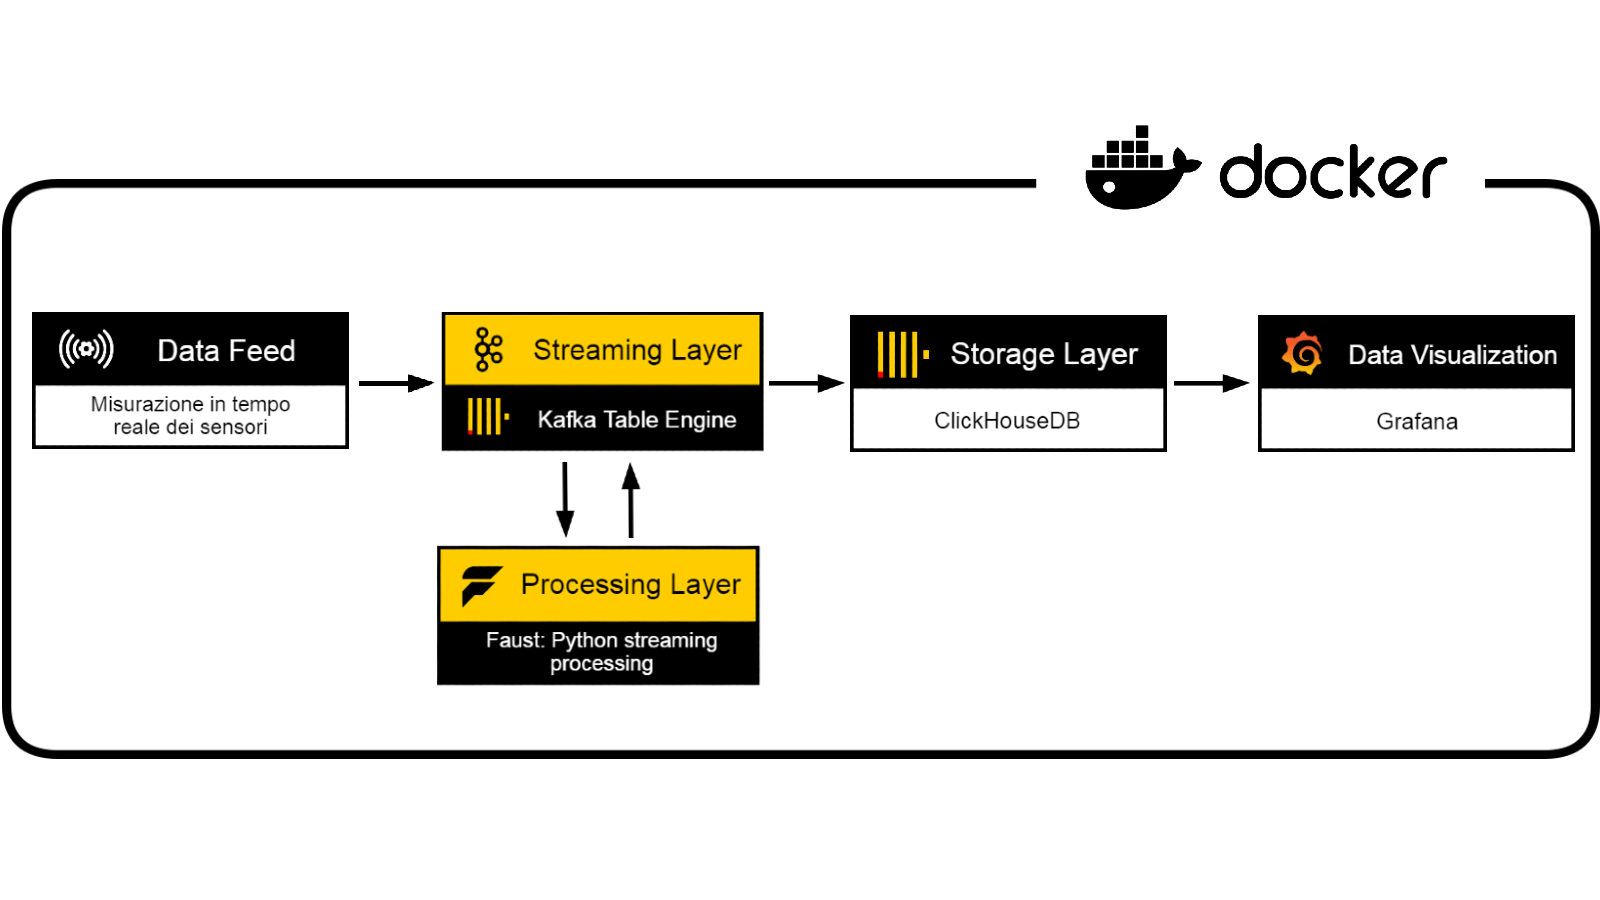
\includegraphics[width=1\textwidth]{../Images/SpecificaTecnica/architettura.jpg}
    \caption{Componenti dell'architettura - innovacity}
    \label{fig: fdf}
\end{figure}

\begin{itemize}
    \item \textbf{Data feed}:Le sorgenti dati sono costituite da sensori IoT dislocati sul territorio cittadino. Questi sensori sono in grado di inviare, ad intervalli regolari, messaggi contenenti misurazioni allo streaming layer;
    \item \textbf{Streaming layer}:Lo streaming layer gestisce i dati in arrivo in tempo reale, per poi archiviarli sistematicamente nello storage layer. Lo streaming Layer è composto da:
    \begin{itemize}
        \item \textbf{Apache Kafka}: Kafka è un sistema di messaggistica distribuito che consente di pubblicare, sottoscrivere e archiviare messaggi in tempo reale. Kafka è utilizzato per ricevere i dati dai sensori IoT e renderli disponibili per l'elaborazione in tempo reale e batch.
        \item \textbf{Clickhouse Kafka table engine}:consumatore che legge i
        dati dal server Kafka per persisterli nello storage layer.
    \end{itemize}
    \item \textbf{Processing Layer:} Il processing Layer è costituito da Faust che consuma i dati dallo streaming layer e li processa in tempo reale. Faust è un framework Python che consente di scrivere applicazioni di streaming in tempo reale. Faust è utilizzato per elaborare i dati in arrivo tramite un modello per il calcolo del punteggio di salute che poi viene reso nuovamente disponibili allo streaming layer.
    \item \textbf{Storage layer}:Lo storage layer è costituito da un database column-oriented, ClickHouse, che archivia i dati in arrivo dallo streaming layer. Questi dati sono disponibili per l'analisi e la visualizzazione in tempo reale e batch.
    \item \textbf{Data Visualization Layer}: composto da Grafana, si occupa della visualizzazione dei dati elaborati ottenuti dallo storage layer e della gestione delle notifiche in caso di anomalie rilevate.
\end{itemize}
\subsection{Architettura dei simulatori} \label{sec:architettura_simulatori}
Nonostante i simulatori non siano ufficialmente considerati parte integrante del prodotto dalla proponente, il nostro team ha scelto di dedicare alcune risorse alla progettazione di questa componente nell'ambito del progetto didattico. Inoltre, abbiamo deciso di implementare e tenere conto delle possibili logiche dei microcontrollori associati ai sensori IoT, che possono effettuare operazioni per rendere più efficiente l'intero sistema.

Nei paragrafi successivi, verrà presentata l'architettura individuata mediante l'utilizzo di diagrammi delle classi e relative descrizioni rapide. Inoltre, saranno motivate le scelte dei design pattern individuati e le decisioni progettuali rilevanti. Successivamente, per ogni classe, saranno illustrati metodi e attributi.
\subsubsection{Modulo simulatori sensori}
\begin{figure}[H]
    \centering
    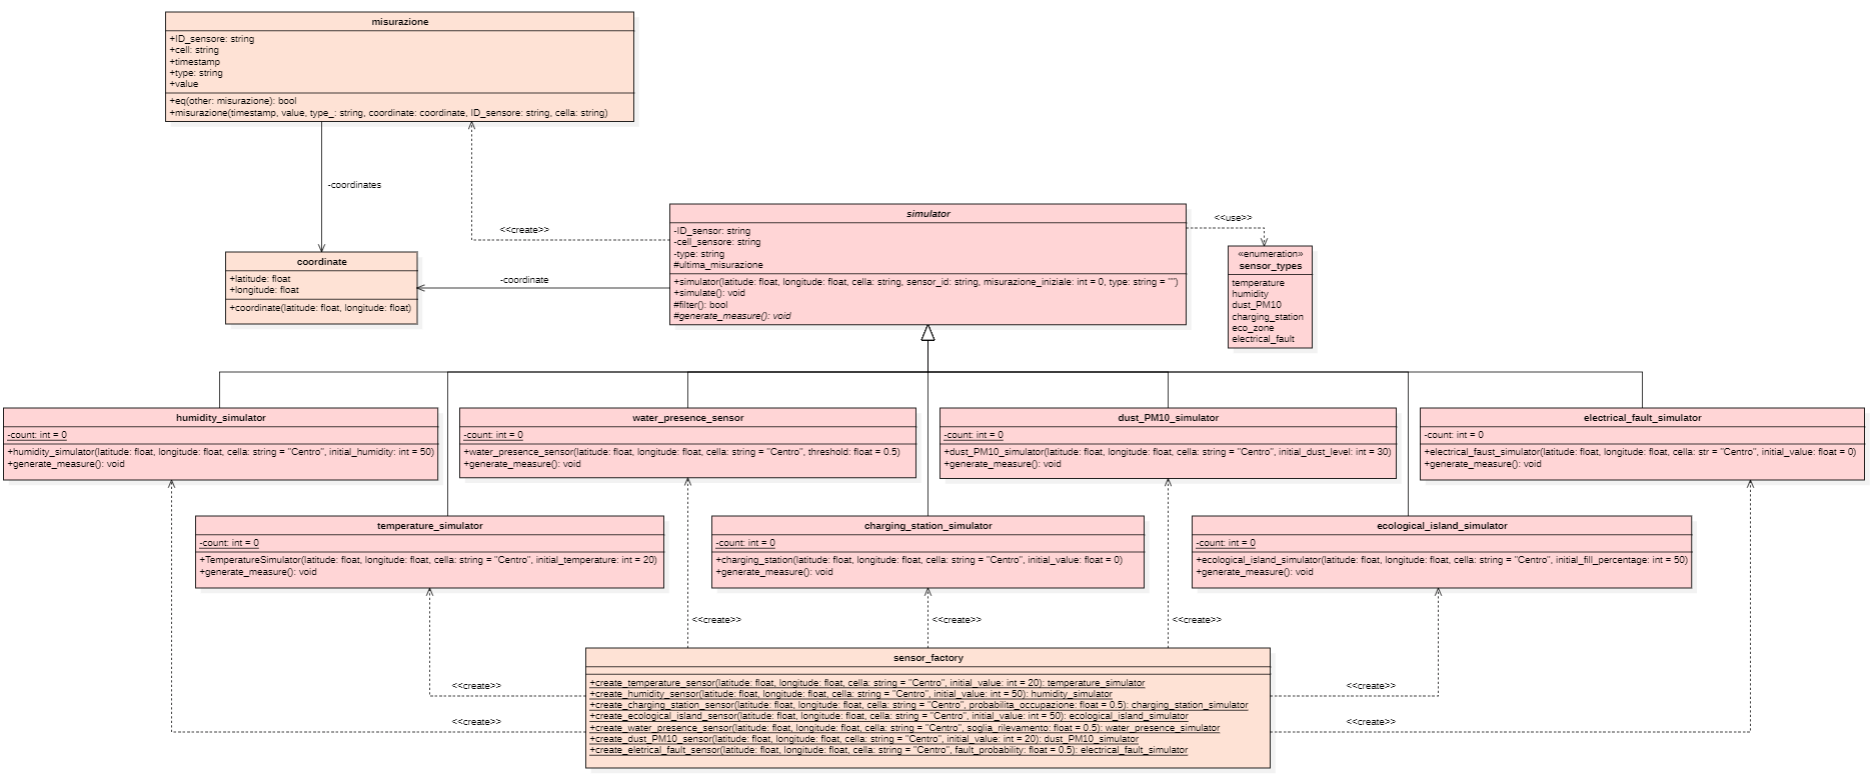
\includegraphics[width=1\textwidth]{../Images/SpecificaTecnica/simulatoriSensori.PNG}
    \caption{Modulo simulatori sensori - innovacity}
    \label{fig: fddf}
\end{figure}
Questo modulo si occupa della generazione di dati di misurazione per diverse tipologie di sensori.

\paragraph{Design pattern Template Method:}

La classe astratta \textit{Simulator} implementa il design pattern \textit{Template Method}. Il metodo \textit{simulate()} fornisce lo scheletro dell'algoritmo per la generazione e la gestione delle misurazioni. Le classi concrete che estendono \textit{Simulator} implementano:
\begin{itemize}
    \item \textbf{Metodo \textit{generate\_measure()}}: per la generazione semi randomica della misurazione associata al tipo di sensore;
    \item \textbf{Metodo \textit{filter()}}: per la logica di filtrazione di misurazioni errate o non attendibili (ad esempio, negative, fuori range o consecutive troppo distanti). Il metodo \textit{filter()} offre un'implementazione di default che lascia passare ogni misurazione senza modifiche.
\end{itemize}

Il design pattern \textit{Template Method} è stato scelto per:
\begin{itemize}
    \item Permettere una facile estensione del sistema con nuovi tipi di sensori che dovranno unicamente implementare la loro logica di generazione delle misurazioni e di filtering se necessario;
    \item Standardizzare i passi per la generazione delle misurazioni, garantendo coerenza e manutenibilità del codice;
    \item Ridurre la duplicazione del codice.
\end{itemize}

Una volta ottenuto lo stato del sensore, esso viene inserito in un oggetto di tipo \textit{Misurazione}. Questo oggetto contiene informazioni di contesto come:
\begin{itemize}
    \item Identificativo del sensore;
    \item Cella della città in cui è presente;
    \item Timestamp della misurazione;
    \item Valore della misurazione;
    \item Coordinate;
    \item Tipologia di misurazione.
\end{itemize}
L'oggetto \textit{Misurazione} viene poi ritornato al chiamante che si occuperà di inviarlo al server \textit{Kafka}.
Un oggetto di tipo \textit{Simulator} verrà assegnato ad ogni \textit{SimulatorThread} che chiamerà ad intervalli regolari il metodo \textit{simulate()} ottenendo appunto la misurazione che invierà al server \textit{Kafka} tramite un modulo apposito e indipendendente.

\paragraph{Design pattern Factory:}
SensorFactory implementa il design pattern \textit{Factory} per la creazione di simulatori dei sensori.
Il pattern FACTORY è un pattern di tipo “Creazionale” secondo la classificazione della GoF.
I pattern di tipo creazionali si occupano della costruzione delle simulazioni dei sensori e delle problematiche che si possono originare, astraggono il processo di creazione degli oggetti, nascondono i dettagli della creazione e rendono i sistemi indipendenti da come gli oggetti sono creati e composti.
Il pattern Factory incapsula la creazione concreta dei sensori, consentendo al client
(l’utilizzatore) di non conoscere i dettagli.


\paragraph{Classi: metodi e attributi}
\begin{itemize}
    \item {\textbf{Classe astratta: \textit{Simulator}}}
        \begin{itemize}
            \item \textbf{Attributi}: 
            \begin{itemize}
                \item \textbf{ID\_sensor:str [private]} - Identificatore univoco del sensore.
                \item \textbf{cella\_sensore:str [private]} - Identificatore della cella del sensore.
                \item \textbf{coordinate:Coordinate [private]} - Coordinate geografiche del sensore.
                \item \textbf{misurazione: T [protected]} - Misurazione corrente del sensore.
                \item \textbf{type:str [private]} - Tipo di sensore.
            \end{itemize}
            \item \textbf{Metodi}:
            \begin{itemize}
                \item \textbf{simulate():Misurazione [public]} - Metodo principale per simulare la generazione di una misurazione.
                Si basa sul design pattern Template Method:
                \begin{enumerate}
                    \item     Chiama generate\_measure() per generare un valore di misurazione.
                    \item     Verifica con filter() se la misurazione è valida (ripete la generazione finché non lo è).
                    \item     Restituisce un oggetto Misurazione con data e ora corrente, valore misurato, tipo di sensore, coordinate e identificativo del sensore.
                \end{enumerate}
                \item \textbf{generate\_measure():None [protected]} - Metodo astratto da implementare nelle classi concrete per generare un valore di misurazione semi-casuale coerente con la tipolgia di sensore da salvare nell'attributo \textit{misurazione}.
                \item \textbf{filter():bool [protected]} - Metodo di filtro per la validazione della misurazione (implementazione di default che accetta sempre la misurazione). Può essere ridefinito nelle classi concrete per implementare la logica di filtraggio.
            \end{itemize}
            \item \textbf{Note}:
            \begin{itemize}
                \item La classe Simulator è astratta e definisce il comportamento generale della simulazione della misurazione.
                \item Le classi concrete che ereditano da Simulator devono implementare il metodo astratto generate\_measure().
                \item Il metodo filter() può essere ridefinito nelle classi concrete per implementare la logica di validazione specifica del sensore.
            \end{itemize}
        \end{itemize}
        
        
        
        
        \item{\textbf{Enumerazione: \textit{SensorTypes}}}
        \begin{itemize}
            \item \textbf{Costanti}: 
            \begin{itemize}
                \item \textbf{TEMPERATURE:str [public]} - Rappresenta la nomenclatura dei sensore di temperatura.
                \item \textbf{HUMIDITY:str [public]} - Rappresenta la nomenclatura dei sensore di umidità.
                \item \textbf{DUST\_PM10:str [public]} - Rappresenta la nomenclatura dei sensore di "polvere PM10".
                \item \textbf{CHARGING\_STATION:str [public]} - Rappresenta la nomenclatura dei sensore di stato delle colonnine di ricarica.
                \item \textbf{ECOLOGICAL\_ISLAND:str [public]} - Rappresenta la nomenclatura dei sensore di stato riempimento isole ecologica.
                \item \textbf{WATER\_PRESENCE:str [public]} - Rappresenta la nomenclatura dei sensore di presenza d'acqua.
                \item \textbf{ELECTRICAL\_FAULT:str [public]} - Rappresenta la nomenclatura dei sensore di guasti elettrici.
            \end{itemize}

            \item \textbf{Note}:
            \begin{itemize}
                \item L'enumerazione viene utilizzata per centralizzare la gestione della nomenclatura dei tipi di sensori che verrà salvata nelle misurazioni.
            \end{itemize}
        \end{itemize}
        
        
    \item{\textbf{Classe: \textit{TemperatureSimulator}}}
    \begin{itemize}
        \item \textbf{Attributi:}
    \begin{itemize}
        \item \textbf{count:int [private, static]} - Contatore statico per generare un ID univoco per ogni istanza.
    \end{itemize}
    \item\textbf{Metodi}: 
    \begin{itemize}
        \item \textbf{generate\_measure():None [protected]} - Genera una misurazione di temperatura semi-casuale e aggiorna la misurazione corrente.
    \end{itemize}
    \item\textbf{Note}:
    \begin{itemize}
        \item La classe TemperatureSimulator è una classe concreta che eredita dalla classe astratta Simulator.
        \item Il costruttore genera automaticamente un ID sensore univoco per ogni istanza.
    \end{itemize}
\end{itemize}
    \item{\textbf{Classe: \textit{HumiditySimulator}}}
    \begin{itemize}
        \item\textbf{Attributi:}
    \begin{itemize}
        \item \textbf{count:int [private, static]} - Contatore statico per generare un ID univoco per ogni istanza.
    \end{itemize}
    \item \textbf{Metodi}: 
    \begin{itemize}
        \item \textbf{generate\_measure():None [protected]} - Genera una misurazione di umidità semi-casuale e aggiorna la misurazione corrente.
    \end{itemize}
    \item \textbf{Note}:
    \begin{itemize}
        \item La classe HumiditySimulator è una classe concreta che eredita dalla classe astratta Simulator.
        \item Il costruttore genera automaticamente un ID sensore univoco per ogni istanza.
    \end{itemize}
\end{itemize}
    \item{\textbf{Classe: \textit{ChargingStationSimulator}}}
    \begin{itemize}
        \item  \textbf{Attributi}: 
    \begin{itemize}
        \item \textbf{count:int [private, static]} - Contatore statico per generare un ID univoco per ogni istanza.
    \end{itemize}
    \item  \textbf{Metodi}:
    \begin{itemize}
        \item \textbf{generate\_measure():None [protected]} - Genera lo stato della colonnina di ricarica (Occupato: True, Libero: False) basata su una probabilità di transizione.
    \end{itemize}
    \item   \textbf{Note}:
    \begin{itemize}
        \item La classe ChargingStationSimulator è una classe concreta che eredita dalla classe astratta Simulator.
        \item Implementa il metodo astratto generate\_measure() per generare una misurazione basata sulla probabilità di transizione.
        \item Il costruttore genera automaticamente un ID sensore univoco per ogni istanza.
    \end{itemize}
\end{itemize}
    \item{\textbf{Classe: \textit{DustPM10Simulator}}}
    \begin{itemize}
        \item   \textbf{Attributi}: 
    \begin{itemize}
        \item \textbf{count:int [private, static]} - Contatore statico per generare un ID univoco per ogni istanza.
    \end{itemize}
    \item    \textbf{Metodi}: 
    \begin{itemize}
        \item \textbf{generate\_measure():None [protected]} - Genera una variazione di polvere PM10 semi-casuale e aggiorna la misurazione corrente.
    \end{itemize}
    \item    \textbf{Note}:
    \begin{itemize}
        \item La classe DustPM10Simulator è una classe concreta che eredita dalla classe astratta Simulator.
        \item Il costruttore genera automaticamente un ID sensore univoco per ogni istanza.
    \end{itemize}
\end{itemize}
    \item{\textbf{Classe: \textit{ElectricalFaultSimulator}}}
    \begin{itemize}
        \item   \textbf{Attributi}: 
    \begin{itemize}
        \item \textbf{count:int [private, static]} - Contatore statico per generare un ID univoco per ogni istanza.
    \end{itemize}
    \item   \textbf{Metodi}: 
    \begin{itemize}
        \item \textbf{generate\_measure():None [protected]} - Genera lo stato di una centralina elettrica (Guasto verificato: True, Operativa: False) basata sulla probabilità di guasto.
    \end{itemize}
    \item   \textbf{Note}:
    \begin{itemize}
        \item La classe ElectricalFaultSimulator è una classe concreta che eredita dalla classe astratta Simulator.
        \item Il costruttore genera automaticamente un ID sensore univoco per ogni istanza.
    \end{itemize}
\end{itemize}
    \item{\textbf{Classe: \textit{EcologicalIslandSimulator}}}
    \begin{itemize}
        \item    \textbf{Attributi}: 
    \begin{itemize}
        \item \textbf{count:int [private, static]} - Contatore statico per generare un ID univoco per ogni istanza.
    \end{itemize}
    \item    \textbf{Metodi}: 
    \begin{itemize}
        \item \textbf{generate\_measure():None [protected]} - Genera una misurazione della percentuale di riempimento di un isola ecologica.
    \end{itemize}
    \item    \textbf{Note}:
    \begin{itemize}
        \item La classe EcologicalIslandSimulator è una classe concreta che eredita dalla classe astratta Simulator.
        \item Il costruttore genera automaticamente un ID sensore univoco per ogni istanza.
    \end{itemize}
\end{itemize}
    \item{\textbf{Classe: \textit{WaterPresenceSensor}}}
    \begin{itemize}
        \item    \textbf{Attributi}: 
    \begin{itemize}
        \item \textbf{count:int [private, static]} - Contatore statico per generare un ID univoco per ogni istanza.
    \end{itemize}
    \item    \textbf{Metodi}: 
    \begin{itemize}
        \item \textbf{generate\_measure():None [protected]} - Genera una misurazione basata sulla soglia di presenza dell'acqua (Acqua rilevata: True, Acqua non rilevata:False).
    \end{itemize}
    \item    \textbf{Note}:
    \begin{itemize}
        \item La classe EcologicalIslandSimulator è una classe concreta che eredita dalla classe astratta Simulator.
        \item Il costruttore genera automaticamente un ID sensore univoco per ogni istanza.
    \end{itemize}
\end{itemize}
    \item{\textbf{Classe: \textit{Misurazione}}}
    \begin{itemize}
        \item   \textbf{Attributi}: 
    \begin{itemize}
        \item \textbf{timestamp:datetime [private]} - Timestamp della misurazione.
        \item \textbf{value:T [private]} - Valore della misurazione.
        \item \textbf{type:str [private]} - Tipo della misurazione.
        \item \textbf{coordinates:Coordinate [private]} - Coordinate della misurazione.
        \item \textbf{ID\_sensore:str [private]} - ID del sensore che ha effettuato la misurazione.
        \item \textbf{cella:str [private]} - Cella in cui è stata effettuata la misurazione.
    \end{itemize}
    \item   \textbf{Metodi}: 
    \begin{itemize}
        \item \textbf{\_\_eq\_\_(other:Misurazione):bool [public]} - Ridefinizione dell'operatore di uguaglianza per confrontare due oggetti Misurazione.
    \end{itemize}
\end{itemize}
    \item{\textbf{Classe: \textit{Coordinate}}}
    \begin{itemize}
        \item    \textbf{Attributi}: 
    \begin{itemize}
        \item \textbf{latitude:float [private]} - Latitudine della coordinata.
        \item \textbf{longitude:float [private]} - Longitudine della coordinata.
    \end{itemize}
    \item     \textbf{Metodi}: 
    \begin{itemize}
        \item \textbf{\_\_eq\_\_(other:Coordinate):bool [public]} - Ridefinizione dell'operatore di uguaglianza per confrontare due oggetti Coordinate.
    \end{itemize}
\end{itemize}
    \item{\textbf{Classe: \textit{SensorFactory}}}
    \begin{itemize}
        \item    \textbf{Metodi}: 
\begin{itemize}
    \item \textbf{create\_temperature\_sensor(latitude: float, longitude: float, cella: str, initial\_value:float):TemperatureSimulator [public, static]} - Crea un simulatore di temperatura.
    \item \textbf{create\_humidity\_sensor(latitude: float, longitude: float, cella: str, initial\_value:float):HumiditySimulator [public, static]} - Crea un simulatore di umidità.
    \item \textbf{create\_charging\_station\_sensor(latitude: float, longitude: float, cella: str, probabilita\_occupazione:float):ChargingStationSimulator [public, static]} - Crea un simulatore di stazione di ricarica.
    \item \textbf{create\_ecological\_island\_sensor(latitude: float, longitude: float, cella: str, initial\_value:float):EcologicalIslandSimulator [public, static]} - Crea un simulatore di isola ecologica.
    \item \textbf{create\_water\_presence\_sensor(latitude: float, longitude: float, cella: str, soglia\_rilevamento:float):WaterPresenceSensor [public, static]} - Crea un sensore di presenza d'acqua.
    \item \textbf{create\_dust\_PM10\_sensor(latitude: float, longitude: float, cella: str, initial\_value:float):DustPM10Simulator [public, static]} - Crea un simulatore di polvere PM10.
    \item \textbf{create\_eletrical\_fault\_sensor(latitude: float, longitude: float, cella: str, fault\_probability:float):ElectricalFaultSimulator [public, static]} - Crea un simulatore di guasto elettrico.
\end{itemize}
\textbf{Note}:
    \begin{itemize}
        \item Implementazione del Pattern Factory;
        \item Fornisce metodi per la creazione di simulatori di sensori;
        \item Astrae il processo di creazione dei sensori, nascondendo i dettagli della creazione.
    \end{itemize}
\end{itemize}
\end{itemize}




\subsubsection{Modulo Writers}
\begin{figure}[H]
    \centering
    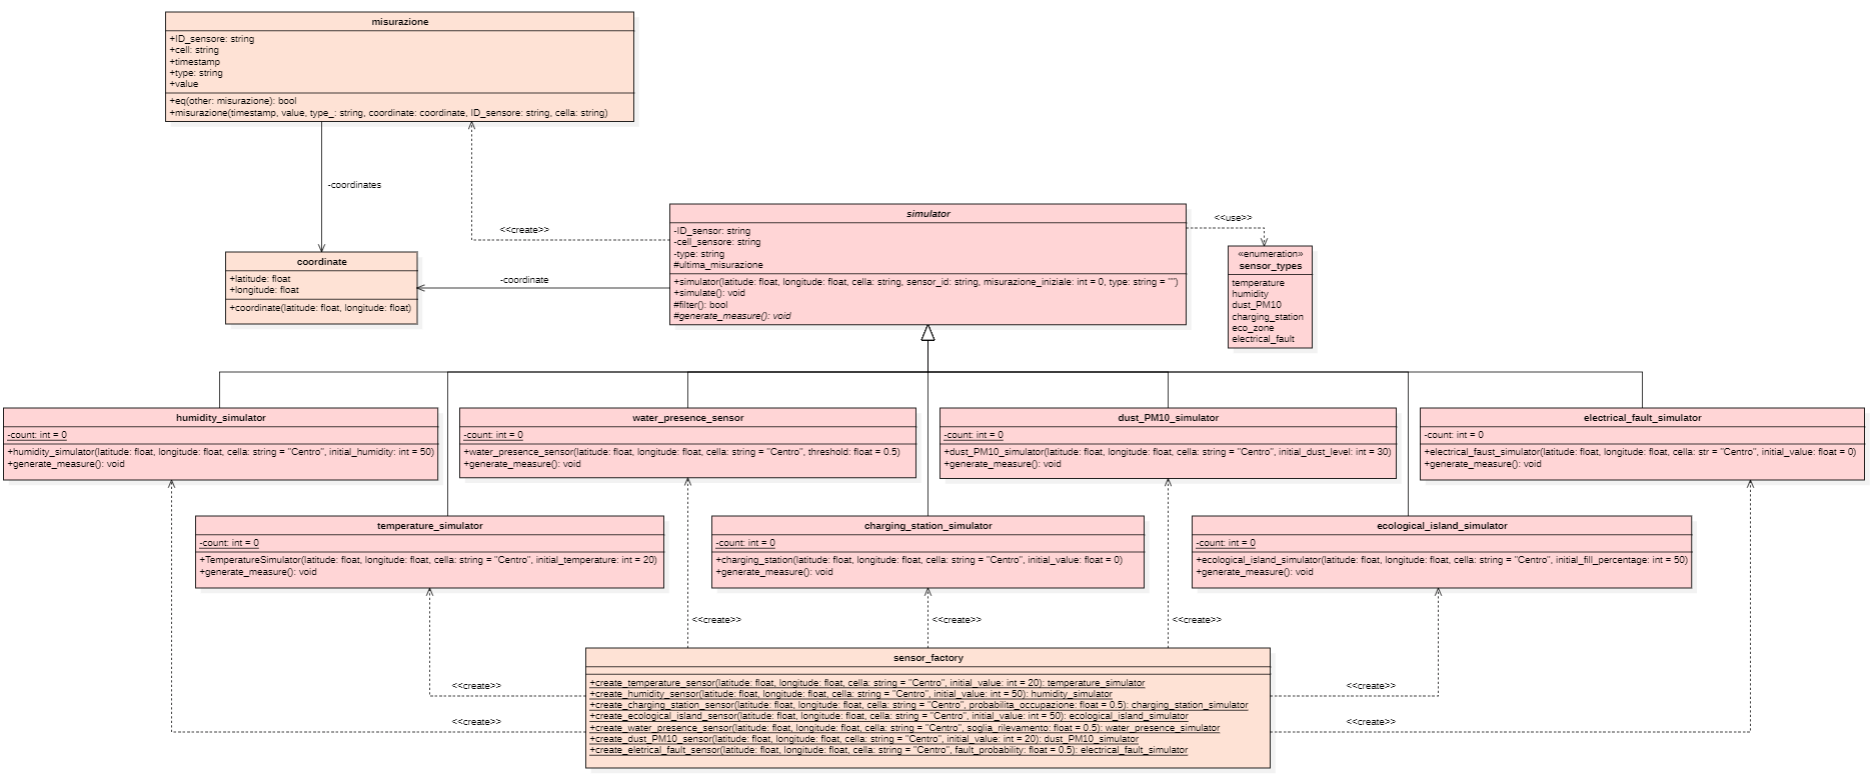
\includegraphics[width=1\textwidth]{../Images/SpecificaTecnica/simulatoriSensori.PNG}
    \caption{Modulo writers - innovacity}
    \label{fig: fdsd}
\end{figure}

Questo modulo si occupa della scrittura e/o invio di informazioni a diverse tipologie di servizi e vuole essere completamentemente indipendendente e non influenzato dal modulo della simulazione dei sensori cosi da poter consentire un suo riutilizzo.

\paragraph{Design pattern Strategy + Composite:}
Il modulo presenta un interfaccia \textit{Writer} che offre il metodo di scrittura \textit{write()} di oggetti di tipo \textit{Writable}.
Questo metodo è implementato da diverse classi concrete che rappresentano i vari servizi a cui è possibile inviare le informazioni.
Questo approccio implementa il design pattern \textit{Strategy} per la scrittura dei dati su diverse piattaforme/servizi e il design pattern \textit{Composite} per la gestione di più servizi a cui scrivere contemporaneamente in modo completamentemente indifferenziato dalla scrittura ad un singolo servizio.
Nello specifico sono state implentate tre strategie di scrittura:la prima, (\textit{KafkaWriter}), atta a permettere al simulatore di inviare messaggi a Kafka,  la seconda (\textit{StdOutWriter}) atta a permettere di stampare i \textit{Writable}su terminale e la terza (\textit{ListWriter}) per il salvataggio su una lista degli oggetti \textit{Writable}.
L'utilizzo del design pattern Composite e Strategy in questo caso ha diverse motivazioni:
\begin{itemize}
    \item \textbf{Gestione uniforme dei servizi}: Il pattern Strategy consente di definire una famiglia di algoritmi, incapsularli e renderli intercambiabili. In questo caso, i servizi di scrittura sono trattati come algoritmi intercambiabili, consentendo di scrivere informazioni su diversi servizi senza dover conoscere i dettagli di implementazione di ciascuno.
    \item \textbf{Gestione gerarchica dei servizi}: Il pattern Composite consente di trattare gli oggetti singoli e le loro composizioni (gruppi di oggetti) allo stesso modo. Nel contesto del modulo, potrebbe esserci la necessità di gestire non solo singoli servizi, ma anche gruppi di servizi. Ad esempio, potrebbe essere utile inviare informazioni contemporaneamente a diversi servizi, come un database, un file di log e un servizio di notifica. Il Composite consente di comporre questi servizi in modo gerarchico e trattarli uniformemente.
\end{itemize}

\paragraph{Design pattern Object Adapter:}
Nello specifico, la classe \textit{KafkaWriter} realizza la sua funzionalità attraverso l'utilizzo del design pattern \textit{Adapter}, nella sua variante \textit{Object Adapter}. Tale scelta è stata motivata dall'impiego della classe \textit{Producer} della libreria \textit{confluent\_kafka}, la quale potrebbe subire variazioni non controllabili da noi. Per garantire la capacità di rispondere prontamente a tali cambiamenti senza dover modificare la classe \textit{KafkaWriter} o altri parti di sistema, si è optato per l'utilizzo di questo pattern, trasferendo così la complessità derivante da tali modifiche proprio nell'adapter.
Inoltre grazie all'interfaccia \textit{KafkaTarget}, si è garantita la possibilità di estendere il sistema con nuovi metodi di scrittura su Kafka o l'utilizzo di nuove librerie senza dover modificare la classe \textit{KafkaWriter} ma solamente aggiungendo una nuova classe adapter che implementi \textit{KafkaTarget}.



\paragraph{Classi: metodi e attributi}

\begin{itemize}
    \item{\textbf{Interfaccia: \textit{Writable}}}
    \begin{itemize}
        \item\textbf{Metodi}: 
        \begin{itemize}
            \item \textbf{to\_json(): [public, abstract]} - Metodo astratto che deve essere implementato nelle sottoclassi per convertire l'oggetto in una stringa JSON.
        \end{itemize}
        \item\textbf{Note}:
        \begin{itemize}
            \item L'interfaccia \textit{Writable} definisce un insieme di metodi che una classe deve implementare perchè possa essere utilizzata dalle strategie di scrittura.
        \end{itemize}
    \end{itemize}
    \item{\textbf{Interfaccia: \textit{Writer}}}
     \begin{itemize}
        \item \textbf{Metodi:}
         \begin{itemize}
            \item \textbf{write(to\_write: Writable): None [public, abstract]} - Metodo astratto che deve essere implementato nelle sottoclassi per scrivere un oggetto Writable.
        \end{itemize}
        \item\textbf{Note}:
        \begin{itemize}
            \item L'interfaccia \textit{Writer} definisce un insieme di metodi che una classe deve implementare perchè possa essere utilizzata come strategia di scrittura;
            \item Rappresenta l'interfaccia "Component" del pattern \textit{Composite} che descrive le operazioni comuni sia agli elementi semplici che a quelli complessi dell'albero.
        \end{itemize}
    \end{itemize}
    \item{\textbf{Classe: \textit{StdoutWriter}}}
    \begin{itemize}
    \item\textbf{Attributi}:
        \begin{itemize}
        \item \textbf{lock:threading.Lock [private]} - Lock per garantire l'accesso esclusivo alla stampa ed un esecuzione Thread safe.
    \end{itemize}
    \item \textbf{Metodi: }
    \begin{itemize}
        \item \textbf{write(to\_write: Writable): None [public]} - Stampa l'oggetto Writable come stringa JSON nella console;
    \end{itemize}
    \item\textbf{Note}:
        \begin{itemize}
            \item La classe è una strategia di scrittura del pattern \textit{Strategy} ma anche la componente "Leaf" del pattern \textit{Composite}, ovvero l'elemento base che non ha sottoelementi.
        \end{itemize}
    \end{itemize}
    \item{\textbf{Classe: \textit{ListWriter}}}
    \begin{itemize}
    \item\textbf{Attributi}:
        \begin{itemize}
        \item \textbf{data\_list:list [private]} - Lista per memorizzare gli oggetti Writable.
        \item \textbf{lock:threading.Lock [private]} - Lock per garantire l'accesso esclusivo alla lista ed un esecuzione Thread safe.
    \end{itemize}
    \item \textbf{Metodi: }
    \begin{itemize}
        \item \textbf{write(to\_write: Writable): None [public]} - Aggiunge l'oggetto Writable alla lista.
        \item \textbf{get\_data\_list(): list [public]} - Restituisce la lista di oggetti Writable.
    \end{itemize}
    \item\textbf{Note}:
        \begin{itemize}
            \item La classe è una strategia di scrittura del pattern \textit{Strategy} ma anche la componente "Leaf" del pattern \textit{Composite}, ovvero l'elemento base che non ha sottoelementi.
        \end{itemize}
    \end{itemize}
    \item{\textbf{Classe: \textit{KafkaWriter}}}
    \begin{itemize}
    \item\textbf{Attributi}:
        \begin{itemize}
        \item \textbf{lock:threading.Lock [private]} - Lock per garantire l'accesso esclusivo alla scrittura su Kafka ed un esecuzione Thread safe.
        \item \textbf{kafka\_target:KafkaTarget [private]} - Riferimento ad un implementazione di KafkaTarget per effettuare l'effettiva scrittura in Kafka tramite librerie.
    \end{itemize}
    \item \textbf{Metodi: }
    \begin{itemize}
        \item \textbf{write(to\_write: Writable): None [public]} - Scrive l'oggetto Writable come stringa JSON su Kafka.
    \end{itemize}
    \item\textbf{Note}:
        \begin{itemize}
            \item La classe è una strategia di scrittura del pattern \textit{Strategy} ma anche la componente "Leaf" del pattern \textit{Composite}, ovvero l'elemento base che non ha sottoelementi.
            \item La costruzione dell'oggetto KafkaWriter richiede un riferimento ad un oggetto che implementi l'interfaccia KafkaTarget.
        \end{itemize}
    \end{itemize}
    \item{\textbf{Classe: \textit{CompositeWriter}}}
    \begin{itemize}
    \item\textbf{Attributi}:
        \begin{itemize}
        \item \textbf{writers:Writer* [protected]} - Lista di oggetti Writer.
    \end{itemize}
    \item \textbf{Metodi: }
    \begin{itemize}
        \item \textbf{add\_writer(writer: Writer): CompositeWriter [public]} - Aggiunge un oggetto Writer alla lista di writers.
        \item \textbf{add\_kafkaConfluent\_writer(topic: str, host: str, port: int): CompositeWriter [public]} - Crea un KafkaWriter con un KafkaConfluentAdapter e lo aggiunge alla lista di writers.
        \item \textbf{add\_stdOut\_writer(): CompositeWriter [public]} - Crea un StdoutWriter e lo aggiunge alla lista di writers.
        \item \textbf{add\_list\_writer(writer\_list: ListWriter): CompositeWriter [public]} - Aggiunge un ListWriter alla lista di writers.
        \item \textbf{remove\_writer(writer: Writer): None [public]} - Rimuove un Writer dalla lista di writers.
        \item \textbf{write(to\_write: Writable): None [public]} - Chiama il metodo write su ogni Writer nella lista di writers passando come attributo il \textit{Writable} ricevuto.
    \end{itemize}
    \item\textbf{Note}:
        \begin{itemize}
            \item La classe è la componente "Composite" del pattern \textit{Composite}, ovvero l'elemento che può avere sottoelementi;
            \item Dopo aver ricevuto una richiesta, il contenitore (detto compisite) delega il lavoro ai suoi sottoelementi:foglie o altri contenitori.
        \end{itemize}
    \end{itemize}
    \item{\textbf{Interfaccia: \textit{KafkaTarget}}}
    \begin{itemize}
    \item \textbf{Metodi: }
    \begin{itemize}
        \item \textbf{write\_to\_kafka(data: str): None [public, abstract]} - Metodo astratto che deve essere implementato nelle sottoclassi per scrivere dati su Kafka.
    \end{itemize}
    \item\textbf{Note}:
        \begin{itemize}
            \item La classe è una interfaccia che fornisce un contratto per le operazioni di scrittura e invio a Kafka.
            \item Rappresenta il componente Target del pattern \textit{Object Adapter}.
        \end{itemize}
    \end{itemize}
\end{itemize}
\subsubsection{Modulo Threading/Scheduling}


\paragraph{Classi: metodi e attributi}





\subsection{Configurazione Database}
Si è optato per l'utilizzo di ClickHouse per il salvataggio dei dati, le motivazioni sono descritte nella sezione \ref{sec:clickHouse}. In particolare, per ogni sensore dei quali si desidera memorizzare i dati, viene creata una tabella che acquisisce i dati dal relativo topic Kafka.
Le tipologie di sensori cui misurazioni si vogliono trattare nel progetto sono:
\begin{itemize}
    \item Sensori di temperatura;
    \item Sensori di umidità;
    \item Sensori di rilevamento polveri sottili; 
    \item Sensori stato riempimento isole ecologiche;
    \item Sensori di stato occupazione colonnine di ricarica;
    \item Sensori di guasti elettrici;
    \item Sensori del livello dell'acqua.
\end{itemize}

La configurazione del database ClickHouse è stata cruciale nella progettazione, poiché un'adeguata ottimizzazione consente di garantire prestazioni ottimali per un sistema orientato al tempo reale e in grado di gestire analisi su enormi volumi di dati.


\subsubsection{Funzionalità Clickhouse utilizzate}
\paragraph{Materialized Views}
Le Materialized Views in ClickHouse sono un meccanismo potente per migliorare le prestazioni delle query e semplificare l'accesso ai dati. Funzionano mantenendo una copia fisica dei risultati di una query di selezione, che viene quindi memorizzata su disco. Questa copia è aggiornata periodicamente in base ai dati sottostanti.

\paragraph*{Utilizzi Principali delle Materialized Views}
\begin{itemize}
    \item \textbf{Calcolo aggregazioni e popolamento tabelle}:Spesso le delle materialized Views sono state utilizzate per calcolare aggregazioni su dati e quindi popolare altre tabelle con i risultati aggregati. Ad esempio, nel caso specifico in cui una Materialized View calcola la media delle temperature per ogni sensore ogni secondo, i risultati di questa vista possono essere utilizzati per popolare una tabella principale contenente i dati di temperatura aggregati, aggiornando i valori di temperatura medi per ogni sensore ogni secondo;
    \item \textbf{Ottimizzazione delle Prestazioni}: memorizzando i risultati di una query complessa, le Materialized Views consentono di eseguire rapidamente le Query successive senza dover ricalcolare i dati ogni volta. Ciò è particolarmente utile in applicazioni che richiedono interrogazioni frequenti su grandi volumi di dati;
    \item \textbf{Decomposizione delle \textit{Query} Complesse}: le Materialized Views consentono di decomporre query complesse in passaggi più semplici e riutilizzabili, migliorando la leggibilità del codice e semplificando lo sviluppo e la manutenzione delle query.
\end{itemize}



\paragraph{MergeTree}\label{sec:MergeTree}
Link alla documentazione: \href{https://clickhouse.com/docs/en/engines/table-engines/mergetree-family/mergetree#mergetree}{ClickHouse - MergeTree}.\newline
MergeTree è uno dei motori di tabella più potenti e utilizzati in ClickHouse, noto per la sua capacità di gestire e memorizzare grandi volumi di dati in modo efficiente. È una scelta ideale per applicazioni che richiedono l'archiviazione e l'analisi di dati cronologicamente ordinati, come i dati di log o di monitoraggio. L'architettura di MergeTree organizza i dati in parti, ciascuna contenente una serie di punti dati ordinati cronologicamente. Questa organizzazione ottimizzata consente di eseguire rapidamente le query che richiedono l'accesso a dati specifici all'interno di un intervallo di tempo definito, garantendo prestazioni elevate anche su grandi dataset. Oltre alla gestione efficiente dei dati, MergeTree supporta funzionalità avanzate come la compressione dei dati e la gestione automatica delle partizioni. Queste caratteristiche consentono di ottimizzare ulteriormente le prestazioni e la gestione complessiva dei dati, rendendo MergeTree una scelta affidabile per una vasta gamma di scenari di utilizzo in ClickHouse.



\paragraph{Time To Live in ClickHouse} \label{sec:RollupTTL}
Link alla documentazione: \href{https://clickhouse.com/docs/en/guides/developer/ttl#implementing-a-rollup}{ClickHouse - Implementing a Rollup}\newline
In ClickHouse, la funzionalità TTL (Time To Live) è un elemento chiave per gestire grandi volumi di dati in modo efficiente e garantire la pulizia automatica di informazioni obsolete o non più rilevanti. \\
Quando si specifica il motore Rollup per definire una tabella in ClickHouse, si abilita la creazione di tabelle che supportano il TTL. Questo consente di impostare un periodo temporale dopo il quale i dati saranno eliminati automaticamente dalla tabella. La struttura a Rollup organizza i dati in parti, ciascuna contenente una serie di punti dati ordinati cronologicamente. Il TTL può essere configurato per ciascuna parte dei dati, offrendo un controllo preciso sulla conservazione delle informazioni nel tempo. Questa flessibilità è particolarmente utile per applicazioni che richiedono la conservazione di dati storici per un periodo limitato, come ad esempio i dati di log o di monitoraggio. \newline
Un esempio di come potrebbe può venire utilizzato il motore Rollup per il TTL in ClickHouse è il seguente:
\begin{verbatim}
    TTL toDateTime(timestamp) + INTERVAL 1 MONTH
\end{verbatim}
L'uso del TTL di tipo Rollup in questo contesto è cruciale per garantire che la tabella rimanga efficiente e gestibile nel tempo, eliminando automaticamente i dati più vecchi e non più necessari dopo un periodo di tempo specificato. Questo aiuta a ottimizzare le prestazioni complessive del sistema e a gestire in modo efficiente i grandi volumi di dati accumulati nel tempo.


\paragraph{Partition}\label{sec:Partition}
Link alla documentazione: \href{https://clickhouse.com/docs/en/engines/table-engines/mergetree-family/mergetree#partition-by}{ClickHouse - Partitioning}.\\
Le partizioni sono una funzionalità fondamentale di ClickHouse che consente di organizzare in modo efficiente e gestire grandi volumi di dati. Questa caratteristica permette di suddividere i dati in gruppi logici in base a criteri specifici, come il valore di una colonna o un intervallo di tempo. Grazie a questa organizzazione ottimizzata, le query che richiedono l'accesso a dati specifici all'interno di una partizione possono essere eseguite rapidamente, garantendo prestazioni elevate anche su dataset di grandi dimensioni.\\
L'utilizzo delle partizioni nel nostro contesto viene giustificato dall'utilizzo di un TTL (Time To Live), infatti l'utilizzo combinato di queste due funzionalità consente:
\begin{itemize}
    \item Una gestione efficace dei dati nel tempo;
    \item Migliori prestazioni del sistema;
    \item Una semplificazione nella manutenzione del database.
\end{itemize}
Il partizionamento basato sul timestamp è una pratica comune in ClickHouse, poiché consente di organizzare i dati in partizioni in base al periodo temporale, ad esempio mensilmente. Questo approccio ottimizza l'archiviazione e facilita l'analisi dei dati di serie temporali, come le temperature o i log di eventi. Grazie a questa struttura, le query che coinvolgono dati all'interno di specifici intervalli temporali diventano più efficienti, consentendo un accesso rapido e una migliore analisi dei dati.




    
\paragraph{Projection}\label{sec:projections}
Link alla documentazione: \href{https://clickhouse.com/docs/en/sql-reference/statements/alter/projection}{https://clickhouse.com/docs/en/sql-reference/statements/alter/projection}\newline
Le proiezioni memorizzano i dati in un formato che ottimizza l'esecuzione delle \textit{Query}, questa caratteristica è utile per:

\begin{itemize}
    \item Eseguire \textit{Query} su una colonna che non fa parte della chiave primaria;
    \item Pre-aggregare colonne, riducendo sia i calcoli che l'I/O.
\end{itemize}

Puoi definire una o più proiezioni per una tabella e durante l'analisi della \textit{Query} la proiezione con meno dati da esaminare sarà selezionata da ClickHouse senza modificare la \textit{Query} fornita dall'utente.

\paragraph*{Utilizzo dello spazio su disco}
\textbf{Attenzione:} le proiezioni creeranno internamente una nuova tabella nascosta, ciò significa che saranno necessari più I/O e spazio su disco. Ad esempio, se la proiezione ha definito una chiave primaria diversa, tutti i dati dalla tabella originale verranno duplicati.

\subsubsection{Integrazione tramite Kafka Engine in ClickHouse}
ClickHouse supporta l'integrazione con Kafka tramite Kafka Engine, permettendo la lettura dei dati da un topic Kafka e il loro salvataggio in una tabella ClickHouse. Tale funzionalità riveste un'importanza notevole per applicazioni che richiedono l'elaborazione in tempo reale di dati provenienti da fonti esterne, una necessità frequente nel contesto del monitoraggio urbano. L'integrazione con Kafka consente l'acquisizione e la memorizzazione efficiente dei dati, garantendo prestazioni elevate anche su grandi volumi di dati.\\
Kafka Engine è progettato per il recupero di dati una sola volta. Ciò significa che una volta che i dati vengono interrogati da una tabella Kafka, vengono considerati consumati dalla coda. Pertanto, non si dovrebbero mai selezionare dati direttamente da una tabella di Kafka Engine, ma utilizzare invece una vista materializzata. Una vista materializzata viene attivata una volta che i dati sono disponibili in una tabella di Kafka Engine. Automaticamente sposta i dati da una tabella Kafka a una tabella di tipo MergeTree o Distributed. Quindi, sono necessarie almeno 3 tabelle:
\begin{itemize}
  \item La tabella di origine del motore Kafka;
  \item La tabella di destinazione (famiglia MergeTree o distribuita);
  \item Vista materializzata per spostare i dati;
\end{itemize}
\begin{figure}[H]
  \centering
  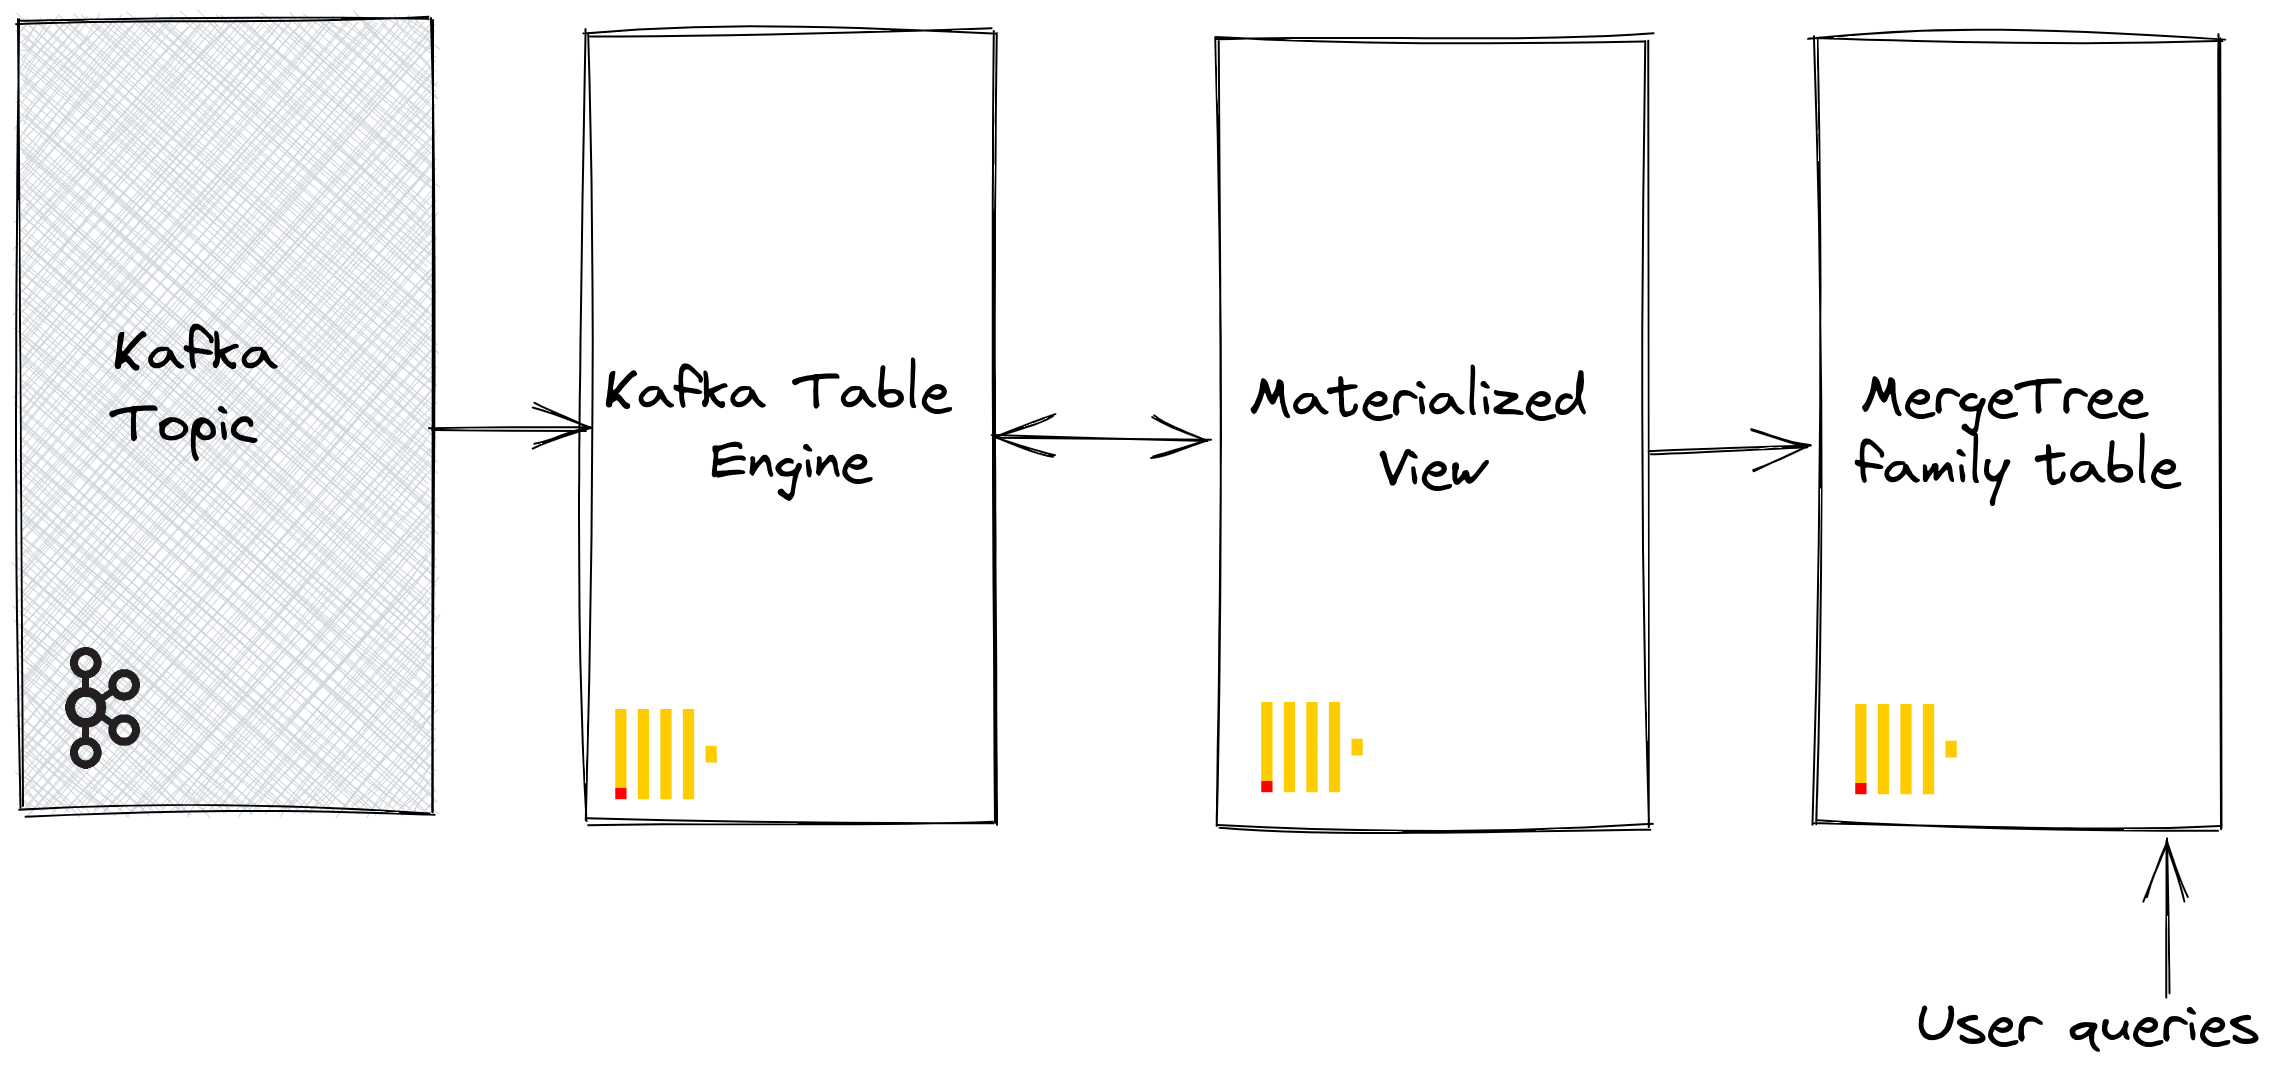
\includegraphics[width=.7\textwidth]{../Images/SpecificaTecnica/kafka_engine_architecture.png}
  \caption{Architettura di Kafka Engine in ClickHouse}
  \label{fig:sensorKafka}
\end{figure}

\subsubsection{Trasferimento dati tramite Materialized View}
Una materialized view funge da ponte tra la fonte dei dati (Kafka Engine) e la destinazione dei dati (MergeTree). Quando nuovi dati vengono scritti nella tabella Kafka Engine, la materialized view viene attivata automaticamente.\\
La materialized view esegue una query sulla tabella Kafka Engine per selezionare i dati più recenti. Una volta selezionati, questi dati vengono inseriti nella tabella di destinazione (ad esempio, una tabella MergeTree). Questo processo avviene in modo automatico e immediato, senza bisogno di intervento manuale.\\
In pratica, la materialized view si assicura che la tabella di destinazione sia sempre aggiornata con i dati più recenti presenti nella tabella Kafka Engine. Questo offre numerosi vantaggi:
\begin{itemize}
  \item \textbf{Automatizzazione del processo}: Non è necessario eseguire manualmente operazioni di trasferimento dati da una tabella all'altra. La materialized view si occupa di tutto in modo automatico;
  \item \textbf{Efficienza}: Il trasferimento dei dati avviene in tempo reale, garantendo che la tabella di destinazione sia sempre allineata con la fonte dei dati senza ritardi;
  \item \textbf{Ottimizzazione delle risorse}: Il processo di trasferimento dei dati è gestito in modo efficiente, utilizzando al meglio le risorse disponibili e garantendo prestazioni elevate.
\end{itemize}
Nel contesto specifico, le materialized view sono responsabili di eseguire controlli sui dati, come ad esempio la verifica della loro correttezza ed affidabilità nel contesto di utilizzo, prima di inserirli nella tabella di destinazione. Questo processo assicura che i dati siano sempre affidabili e pronti per l'analisi, senza la necessità di ulteriori operazioni di pulizia o preparazione.\\
Per esempio, nel caso dei dati di umidità raccolti da sensori in un'area urbana, la materialized view potrebbe eseguire controlli per assicurarsi che i valori rientrino all'interno di un intervallo plausibile e che non ci siano discrepanze improbabili. Ciò garantirebbe che i dati di umidità inseriti nella tabella di destinazione siano accurati e affidabili per l'analisi meteorologica o ambientale.


\subsubsection{Tabella di origine di Kafka Engine per un sensore generico}
Le tabelle del database impiegate per registrare le misurazioni di ciascuna tipologia di sensore presentano una configurazione sostanzialmente simile, differenziandosi principalmente per il tipo di dato della colonna relativa alla misurazione e per il \textit{topic} di riferimento utilizzato per ottenere le misurazioni.
Nello specifico per ogni sensore si avrà la seguente tabella Clickhouse:
\begin{figure}[H]
    \centering
    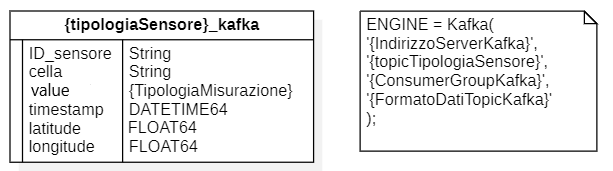
\includegraphics[width=.6\textwidth]{../Images/SpecificaTecnica/sensorType_kafka.PNG}
    \caption{Tabella sensore generico per il reperimento da kafka - ClickHouse}
    \label{fig:sensorKafka}
  \end{figure}

    La tabella è configurata con il motore di storage \textit{Kafka}, il che significa che i dati verranno letti da un \textit{topic Kafka}. 

    I campi sono:
    \begin{itemize}
        \item \textbf{ID\_sensore}: un campo di tipo \textit{String} che identifica univocamente il sensore che ha effettuato la misurazione;
        \item \textbf{cella}: un campo di tipo \textit{String} che rappresenta la cella della città in cui è stata effettuata la misurazione;
        \item \textbf{value}: un campo di tipo variabile a seconda del tipo di misurazione che contiene il valore della temperatura;
        \item \textbf{timestamp}: campo di tipo \textit{DATETIME64} che rappresenta il timestamp della misurazione della temperatura;
        \item \textbf{latitude}: un campo di tipo \textit{Float64} che rappresenta la latitudine del luogo dove è stata effettuata la misurazione;
        \item \textbf{longitude}: un campo di tipo \textit{Float64} che rappresenta la longitudine del luogo dove è stata effettuata la misurazione.
    \end{itemize}

    Mentre i parametri esposti racchiusi da parentesi graffe variano per ogni tipolgia di sensore correlato alla misurazione e sono:
    \begin{itemize}
        \item \textbf{tipologiaSensore}: viene sostituito con la tipologia del sensore che effettua le misurazioni salvate nella tabella; (ex. temperatures)
        \item \textbf{TipoDatoMisurazione}: viene sostituito con il tipo del dato che rappresenta la misurazione (ex. Float32, UInt8);
        \item \textbf{IndirizzoServerKafka}: specifica l'indirizzo del server Kafka.
        Nel nostro caso il server Kafka è in esecuzione su un container \textit{Docker} raggiungibile tramite l'indirizzo:
         \textit{'kafka:9092'};
        \item \textbf{topicTipologiaSensore}: specifica il nome del topic Kafka da cui leggere i dati (ex.temperature);
        \item \textbf{ConsumerGroupKafka}: specifica il nome del consumer group Kafka che verrà utilizzato per leggere i messaggi dal topic \textit{Kafka} denominato 'temperature'.
        Un consumer group in \textit{Kafka} è un gruppo di consumatori che lavorano insieme per consumare i messaggi da uno o più topic. Ogni messaggio inviato a un \textit{topic Kafka} può essere consumato da uno dei consumatori nel gruppo. I consumer all'interno di uno stesso gruppo condividono l'elaborazione dei messaggi all'interno dei topic: ogni messaggio viene elaborato da uno e un solo consumatore all'interno del gruppo. Nel nostro caso sarà sempre '\textit{CG\_Clickhouse\_1}' per indicare il servizio di salvataggio \textit{Clickhouse}.
        \item \textbf{FormatoDatiTopicKafka}: specifica il formato dei dati nel \textit{topic Kafka}. Nel nostro caso, i dati sono nel formato JSONEachRow, che è un formato di serializzazione JSON di \textit{ClickHouse} che consente di scrivere o leggere record JSON separati da una riga. Quindi avremo che <<FormatoDatiTopicKafka>> = JSONEachRow.
        \item \textbf{KafkaSkipBrokenMessages}: specifica il numero di errori da tollerare durante il parsing dei messaggi, configurato a livello di tabella, rappresenta la quantità massima di errori accettabili che il sistema può gestire durante il processo di analisi dei messaggi. Questo parametro consente di regolare il livello di tolleranza agli errori a livello di tabella, offrendo la possibilità di controllare quanto il sistema debba essere flessibile nell'interpretazione dei dati.
    \end{itemize}

    
\subsubsection{Misurazioni temperatura} \label{sec:tab_temperatures}
Di seguito viene fornita la configurazione riguardante il salvataggio delle misurazioni di temperatura:
\paragraph{Tabella: temperatures\_kafka}
\begin{figure}[H]
    \centering
    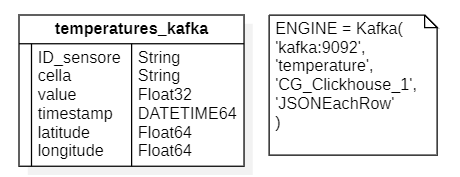
\includegraphics[width=1\textwidth]{../Images/SpecificaTecnica/temperatures_kafka.PNG}
    \caption{Tabella temperatures\_kafka - ClickHouse}
    \label{fig:temperaturesKafka}
  \end{figure}

Il dato della misurazione è di tipo Float32, l'equivalente di float nel linguaggio \textit{C}.
Il topic kafka per ottenere i dati è: \textit{temperature}.

Considerando la possibilità di ricevere molteplici misurazioni dei dati di temperatura all'interno di un singolo secondo di tempo, si procede alla creazione della seguente tabella e alla materialized view correlata, il cui obiettivo è aggregare le misurazioni di temperatura per ridurle ad una singola misurazione per secondo.

\paragraph{Tabella: temperatures}
\begin{figure}[H]
    \centering
    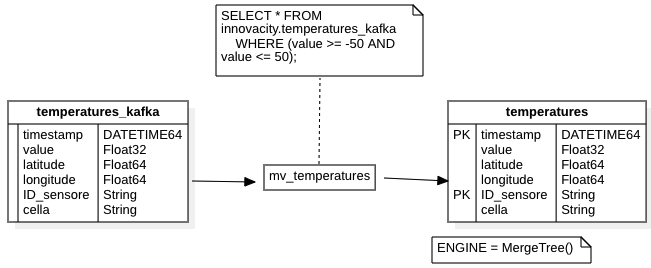
\includegraphics[width=1\textwidth]{../Images/SpecificaTecnica/temperatures.PNG}
    \caption{Tabella temperatures - ClickHouse}
    \label{fig:temperatures}
  \end{figure}

   
    
    \paragraph{Projections per misurazioni di temperatura} \label{sec:temp_projections}
    Durante la fase di progettazione, è stata posta particolare attenzione all'utilizzo delle tabelle appena descritte e alle richieste che verranno formulate su di esse. È emerso, considerando il requisito di suddividere la città in una serie di celle e specificare la cella di origine della misurazione,che la filtrazione delle misurazioni per celle diventerà una richiesta effettuata con frequenza al database.
    Si è giunti quindi all'utilizzo delle \textit{PROJECTIONS}, descritte nella sezione \ref{sec:projections}.
    \vspace{0,3cm}
    \begin{lstlisting}[caption={Esempio di proiezione e materializzazione in una tabella}, captionpos=b]
      --Projection per tabella temperatures
      ALTER TABLE innovacity.temperatures ADD PROJECTION tmp_sensor_cell_projection (SELECT * ORDER BY cella);
      ALTER TABLE innovacity.temperatures MATERIALIZE PROJECTION tmp_sensor_cell_projection;
  \end{lstlisting}
    \vspace{0,3cm}
    La proiezione ci permetterà di filtrare per \textit{cella} e \textit{timestamp} rapidamente, anche se nella tabella originale queste non sOno definite come \textit{PRIMARY\_KEY}.


    \paragraph{Analisi benefici delle Projections}\label{sec:temp_projections_benefici}
    L'aggiunta delle \textit{PROJECTIONS} ha portato risultati di estremo rilievo di seguito esposti.
    Prendendo una \textit{Query} tipo svolta per l'analisi da \textit{Grafana}:
    
    \begin{lstlisting}[caption={Query tipica - Grafana}, captionpos=b]
      SELECT ID_sensore, avgMerge(value) AS value, timestamp
      FROM innovacity.temperatures
      WHERE (cella IN ('Arcella')) AND ((timestamp >= toDateTime64(1708338633507 / 1000, 3)) AND (timestamp <= toDateTime64(1708338933507 / 1000, 3) + INTERVAL 1 DAY))
      GROUP BY timestamp, ID_sensore
      HAVING (value >= -100) AND (value <= 100)

      --Query id: 48635435-9b35-4727-b580-9e33a9db92d4
    \end{lstlisting}

    \begin{figure}[H]
        \centering
        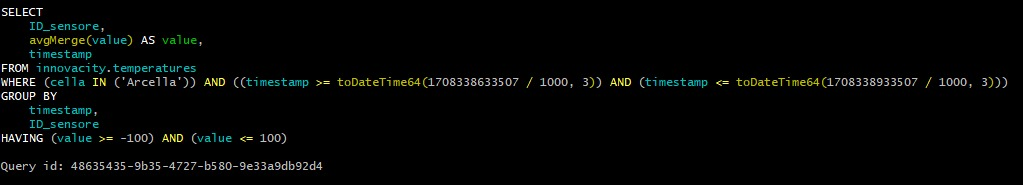
\includegraphics[width=1\textwidth]{../Images/SpecificaTecnica/ProjectionQuery.jpg}
        \caption{Query tipica - Grafana}
        \label{fig:ProjectionsQuery}
      \end{figure}
    senza l'utilizzo delle \textit{PROJECTIONS} il risultato è:
    \begin{figure}[H]
        \centering
        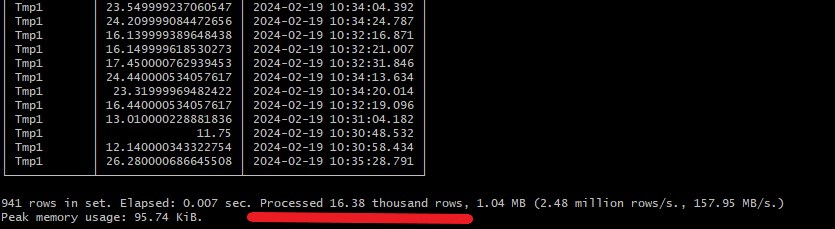
\includegraphics[width=0.9\textwidth]{../Images/SpecificaTecnica/SenzaProectionResult.jpg}
        \caption{Query tipica risultato senza projections}
        \label{fig:ProjectionsQueryWthout}
      \end{figure}
      ovvero sono state processate per ottenere il risultato della \textit{Query} \textbf{16,38 migliaia} di righe.

      Invece in seguito all'aggiunta delle \textit{PROJECTIONS}:
      \begin{figure}[H]
        \centering
        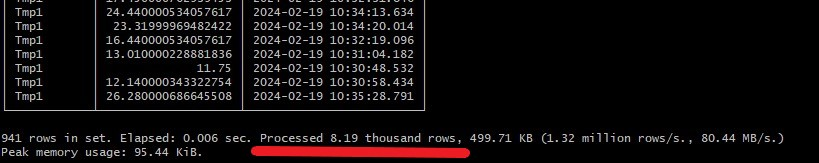
\includegraphics[width=0.9\textwidth]{../Images/SpecificaTecnica/ConProjectionRisultato.jpg}
        \caption{Query tipica risultato con projections}
        \label{fig:ProjectionsQueryWith}
      \end{figure}   
  ovvero sono state processate per ottenere il risultato della \textit{Query} \textbf{8,19 migliaia} di righe, circa la metà rispetto al risultato precedente consentendoci di apprezzare il miglioramento.
Inoltre tramite una \textit{Query} speciale è possibile visualizzare che la \textit{PROJECTIONS} è stata effettivamente utilizzata per ottenere il risultato della \textit{Query} in esame.
\begin{figure}[H]
    \centering
    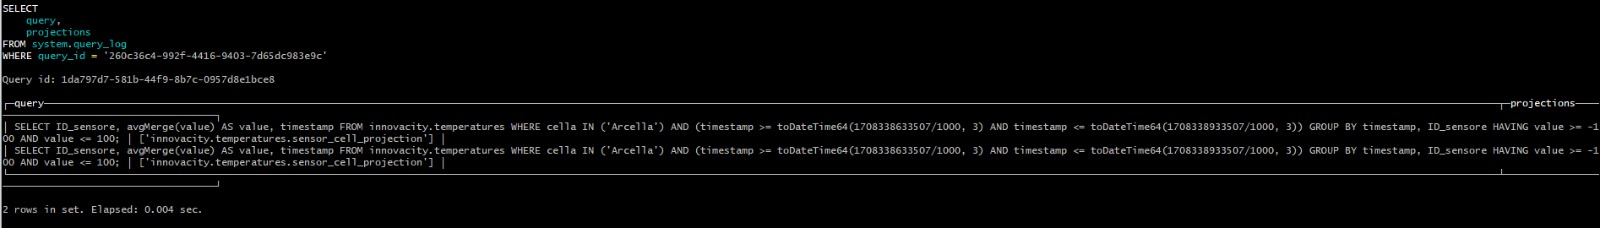
\includegraphics[width=1\textwidth]{../Images/SpecificaTecnica/ProjectionUsedByClickHouse.jpg}
    \caption{Uso della Projection}
    \label{fig:ProjectionsUsed}
\end{figure}

Prendendo in esempio un altra \textit{Query} fatta dall'applicativo dove viene effettuata la media globale di \textbf{170 mila }misurazioni di temperatura si possono apprezzare i benifiici dell'utilizzo delle \textit{PROJECTIONS} e alla fine dell'immagine anche il suo effettivo utilizzo per il calcolo del risultato.
Con l'utilizzo della \textit{PROJECTIONS} abbiamo:
\paragraph{Tabella: humidity\_kafka}
\begin{figure}[H]
    \centering
    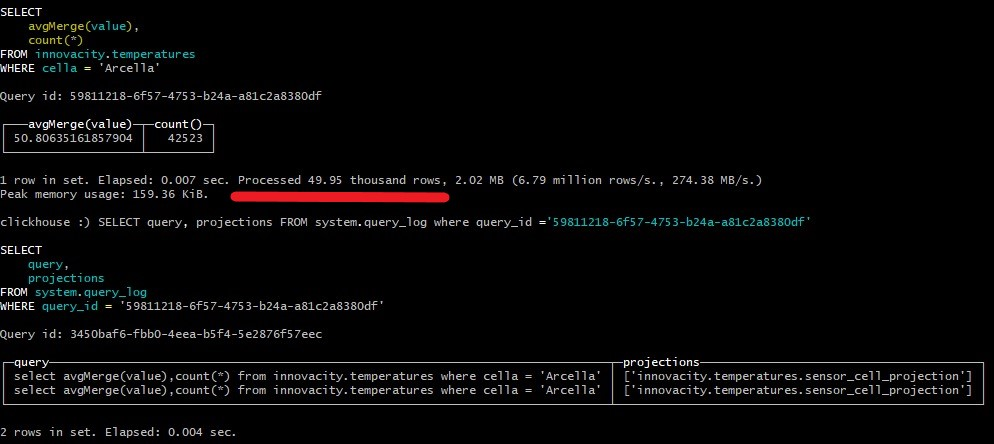
\includegraphics[width=1\textwidth]{../Images/SpecificaTecnica/query2ProjectionsWith.jpg}
    \caption{Query esempio Projection 2 - ClickHouse}
    \label{fig:with2proj}
  \end{figure}
Ovvero il totale di righe processate per ottenere il risultato è di \textbf{49,95 migliaia} con \textbf{0,07 secondi} di tempo utilizzati.
Si puo notare invece la differenza delle righe processate una volta rimossa la \textit{PROJECTIONS}:
\begin{figure}[H]
    \centering
    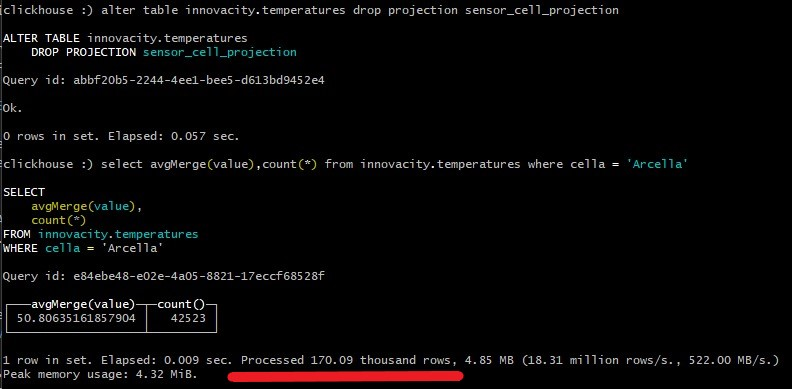
\includegraphics[width=1\textwidth]{../Images/SpecificaTecnica/query2ProjectionsWithout.jpg}
    \caption{Query esempio senza Projection 2 - ClickHouse}
    \label{fig:without2proj}
  \end{figure}

 Il totale di righe processate per ottenere il risultato è ora di \textbf{170,09 migliaia}, ovvero la totalità delle righe presenti nella tabella, con \textbf{0,09 secondi} di tempo utilizzati.

\subsubsection{Misurazioni umidità}
Le considerazioni relative al salvataggio delle misurazioni di umidità coincidono con quelle espresse nella sezione \ref{sec:tab_temperatures} riguardo alle misurazioni di temperatura.
\paragraph{Tabella: humidity\_kafka}
\begin{figure}[H]
    \centering
    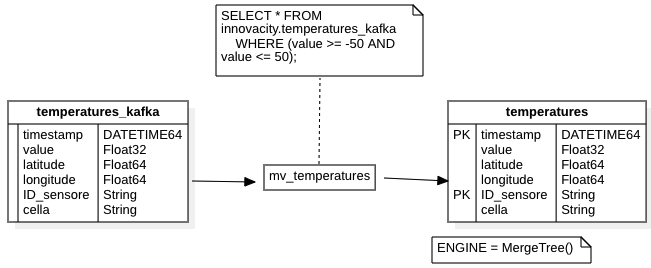
\includegraphics[width=1\textwidth]{../Images/SpecificaTecnica/temperatures.PNG}
    \caption{Tabella humidity\_kafka - ClickHouse}
    \label{fig:umidities_kafka}
  \end{figure}
Il dato della misurazione è di tipo Float32, l’equivalente di float nel linguaggio C. Il topic
kafka per ottenere i dati è: \textbf{humidity}.
\paragraph{Tabella: umidities}
\begin{figure}[H]
    \centering
    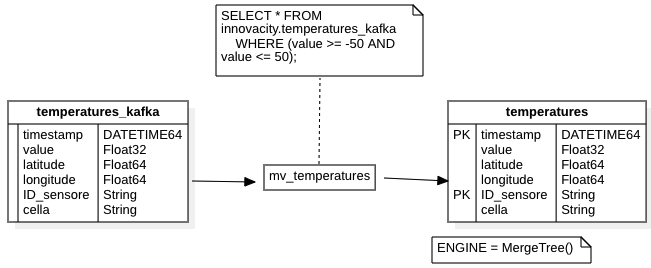
\includegraphics[width=1\textwidth]{../Images/SpecificaTecnica/temperatures.PNG}
    \caption{Tabella humidity - ClickHouse}
    \label{fig:umidities}
  \end{figure}

\paragraph{Projections per misurazioni di umidità} 
Date le stesse considerazioni fatte nella sezione: \ref{sec:temp_projections} anche per le misurazioni di umidità si è deciso di adottare le \textit{PROJECTION}.
I risultati dei benifiici perfettamente riconducibili a quelli per le misurazioni di temperatura alla sezione: \ref{sec:temp_projections_benefici}.

Di seguito vengono fornite le configurazioni delle proiezioni sulle tabelle delle misurazioni di umidità:

\begin{lstlisting}
    --Projection per tabella humidity
    ALTER TABLE innovacity.humidity ADD PROJECTION umd_sensor_cell_projection (SELECT * ORDER BY cella);
    ALTER TABLE innovacity.humidity MATERIALIZE PROJECTION umd_sensor_cell_projection;
\end{lstlisting}


\subsubsection{Misurazioni polveri sottili}Le considerazioni relative al salvataggio delle misurazioni di polveri sottili coincidono con quelle espresse nella sezione \ref{sec:tab_temperatures} riguardo alle misurazioni di temperatura.




\section{Architettura di deployment}
%dubbio che sia corretto
\begin{comment}
    L'architettura di deployment, detta anche "architettura di rilascio", rappresenta la struttura e la configurazione di un sistema software in fase di esecuzione. Essa definisce come i componenti software, i dati e le risorse di rete sono distribuiti e interconnessi nell'ambiente di produzione.
\end{comment}


\subsection{Architettura a microservizi nel IoT}
l modello di architettura dei microservizi è emerso come alternativa alle architetture e alle applicazioni monolitiche, difficili da mantenere ed evolvere a causa dell'elevato accoppiamento tra i loro componenti. Un'architettura a microservizi si basa sul concetto di costruire un'applicazione come un insieme di piccoli servizi interconnessi, che comunicano attraverso protocolli leggeri. Ogni servizio è progettato per svolgere una funzione specifica e può essere sviluppato, testato, deployato e scalato in modo indipendente dagli altri servizi. Questo approccio consente di ottenere una maggiore flessibilità, scalabilità e resilienza rispetto alle architetture monolitiche, consentendo inoltre di adattarsi meglio ai cambiamenti e alle esigenze del business.
Tutti i microservizi di un’applicazione risultano essere completamente separati
tra di loro, e possono essere compilati ed implementati in modo indipendente.
gli altri.
Poiché eseguito in modo del tutto indipendente, ciascun microservizio può essere
aggiornato, distribuito e ridimensionato per rispondere alla richiesta di funzioni
specifiche di un’applicazione. Così, man mano che la domanda per determinati
servizi aumenta, i microservizi possono essere distribuiti su più server e infrastrutture, in base alle esigenze aziendali. In questo modo si possono creare più repliche
solo di quei microservizi che sono soggetti ad un carico lavorativo maggiore, senza
andare a creare una nuova istanza dell’intera applicazione.
Un altro vantaggio viene garantito dall’indipendenza dalla macchina su cui
il microservizio è eseguito. Tale aspetto permette di assegnare diverse potenze
computazionali ai vari microservizi dell’applicazione, andando a bilanciare le risorse
tra i diversi componenti.


Tuttavia, l’architettura a microservizi introduce anche nuove difficoltà. Essendo un sistema composto da più componenti è necessario scegliere e configurare
attentamente le connessioni tra i vari microservizi, talvolta anche introducendo
meccanismi di sicurezza. Inoltre, la fase di testing diventa molto più complicata
rispetto a quella nelle applicazioni monolitiche. Occorre ricordare che un errore in
una parte dell’architettura potrebbe causare un errore in un componente a vari
passi di distanza, a seconda del modo in cui i servizi sono strutturati per supportarsi
a vicenda.
Anche la fase iniziale di installazione dell’applicazione risulta essere più critica.
Per semplificare il deployment, occorre innanzitutto investire notevolmente in
soluzioni di automazione. La complessità dei microservizi renderebbe il deployment
manuale estremamente difficile.
È proprio la natura distribuita di queste applicazioni che rende più complessa
la loro gestione e analisi. In questo tipo di architettura, ad una singola richiesta
corrisponde un lungo percorso all’interno della rete dei microservizi. Se si dovesse
riscontare un eventuale errore o bug, risulta quindi complicato andare ad identificare
quale tra le varie componenti coinvolte ha riportato dei malfunzionamenti. Per
questo motivo è diventato sempre più importante lo sviluppo di piattaforme di
monitoraggio, che sono in grado di tracciare tutte le comunicazioni effettuate e
controllare il corretto funzionamento dei singoli microservizi.
\paragraph*{Perchè l'architettura a microservizi?}
La decisione di adottare un'architettura a microservizi è stata motivata dalla necessità di creare una struttura modulare e scalabile. L'applicazione è stata suddivisa in una suite di microservizi, ciascuno dei quali può essere sviluppato, modificato, deployato e scalato indipendentemente dagli altri.

L'architettura a microservizi si rivela una scelta solida nell'ambito dell'IoT, poiché si prevede che le diverse parti del sistema evolveranno in maniera indipendente nel tempo e poiché la scalabilità e l'isolamento dei guasti sono un aspetto critico. Questa scelta garantisce maggiore flessibilità e prestazioni ottimizzate mediante un utilizzo accurato delle risorse disponibili.

Infatti, nel contesto dell'architettura a microservizi, si presenta l'opportunità di assegnare risorse specifiche a ciascun servizio, il che permette loro di scalare in modo differenziato in base alle necessità. Questo è particolarmente vantaggioso in scenari in cui i servizi potrebbero essere sottoscritti a specifici topic e argomenti all'interno di un sistema di streaming come Kafka.

L'allocazione di risorse individualizzate consente ai servizi di adattarsi dinamicamente alla loro attività e al volume di dati con cui devono interagire. Ad esempio, un servizio che riceve un alto flusso di dati da un particolare topic potrebbe richiedere una maggiore capacità di calcolo e di memorizzazione rispetto a un altro servizio che gestisce un carico meno intenso.

Inoltre, questa flessibilità nell'allocazione delle risorse consente di ottimizzare l'efficienza complessiva del sistema, garantendo che le risorse siano allocate in modo proporzionale alla richiesta effettiva dei servizi. Ciò contribuisce a migliorare le prestazioni complessive del sistema e a garantire una gestione ottimale delle risorse disponibili.

\subsection{Messaggistica nei scenari IoT}
Nelle città intelligenti, dove vengono ricevuti grandi quantità di eventi, abbiamo bisogno di una componente software che faciliti le comunicazioni e la gestione dei dati di input. In tale ambito è utile utilizzare un broker di messaggi. I broker di messaggi consentono di mantenere completamente disaccoppiati l'origine e la destinazione dei messaggi attraverso l'implementazione di un meccanismo di comunicazione asincrono. Consentono inoltre di archiviare i messaggi nel broker finché non possono essere elaborati dal componente di destinazione, nonché da altre funzionalità di gestione. Ogni broker, infatti, offre una serie di funzionalità per la comunicazione, sia attraverso code di messaggi standard, sia attraverso un meccanismo di pubblicazione/sottoscrizione che fa uso di topic; questi sono i due modelli più utilizzati. Tra i vantaggi derivanti dall'utilizzo delle code di messaggi possiamo citare la loro capacità di implementare un algoritmo di bilanciamento del carico. Nel caso degli argomenti dei messaggi, ogni messaggio pubblicato può essere elaborato da tutti i consumatori iscritti a quell'argomento.

\paragraph{Apache Kafka e Schema Registry}
Come gia esposto in precedenza, per la gestione dei dati in streaming è stato scelto Apache Kafka, un sistema di messaggistica distribuito che offre un'architettura a bassa latenza e ad alta affidabilità. Kafka è stato progettato per gestire flussi di dati in tempo reale e per garantire la scalabilità e la tolleranza ai guasti. Inoltre, offre un'API di alto livello per la gestione dei flussi di dati, consentendo di scrivere applicazioni che possono elaborare i dati in tempo reale. Queste caratteristiche lo rendono particolarmente adatto per l'elaborazione dei dati in tempo reale nei contesti IoT, in cui è necessario gestire grandi quantità di dati provenienti da diverse fonti e garantire una bassa latenza e un'elevata affidabilità.

Inoltre l'utlizzo dello Schema Registry permette la definizioni di contratti su cui fanno affidamento produttori e consumatori di dati, garantendo la compatibilità tra le diverse versioni dei messaggi e la corretta interpretazione dei dati da parte dei consumatori. Questo è particolarmente utile in scenari in cui i dati vengono prodotti e consumati da diverse applicazioni e componenti, garantendo che i dati siano correttamente interpretati e che le applicazioni siano in grado di elaborarli in modo coerente.


\subsection{Il container deployment}
Con la tecnica della virtualizzazione leggera, viene implementato un livello di
isolamento a livello software offerto dal sistema
operativo stesso. Nascono così i container, delle unità standard di software che includo il
codice e tutte le sue dipendenze cosicché l’applicazione possa girare velocemente e
in maniera affidabile da un computer ad un altro.
Un progetto completamente open source che ancora oggi continua a perfezionare
la struttura dei container è Docker. Docker implementa un nuovo livello di
astrazione all’interno del sistemo operativo, introducendo una semplicissima gestione
dei container.
Docker ha anche sviluppato quelle che sono chiamate Docker Images, ovvero dei
pacchetti eseguibili di software, leggeri ed indipendenti, che includono tutto ciò di
cui ha bisogno l’applicazione per essere eseguita correttamente: codice, runtime,
tools di sistema, librerie di sistema e impostazioni. I Docker Image diventano
container una volta eseguiti dalla Docker Engine, una piattaforma che consente alle applicazioni containerizzate di essere eseguite ovunque in modo coerente su
qualsiasi infrastruttura, eliminando il problema dalle dipendenze software.
Al giorno d’oggi i Docker Container sono la soluzione migliore per gestire più
applicazioni su uno stesso server contemporaneamente, poiché non richiedono un
sistema operativo per applicazione. Inoltre, condividendo il kernel del sistema
operativo su cui sono in esecuzione risultano estremamente leggeri e molto più
veloci delle macchine virtuali.


Per implementare l'intero stack tecnologico e i layer di elaborazione dati in streaming, è stato configurato un ambiente Docker a microservizi che simula la divisione e la distribuzione dei layer e dei servizi. In particolare, sono stati creati container per:
\begin{itemize}
    \item \textbf{Data feed (Fonti di dati:)}:
    \begin{itemize}
        \item \textbf{Simulators}: Esegue i \textbf{simulatori di sensori} per la raccolta dei dati.
        \item Produce dati nel formato JSON definito nello Schema Registry;
        \item Non espone porte all’esterno.
    \end{itemize} 
    \item \textbf{Streaming layer}:
    \begin{itemize}
        \item Esegue \textbf{Apache Kafka} per la gestione del flusso di dati in tempo reale.
        \item Accessibile agli altri container tramite l'indirizzo \textit{\textbf{kafka:9092}}.
        \item Kafka facilita la comunicazione asincrona e disaccoppiata tra i microservizi.
        \item Permette ai microservizi di comunicare in modo indipendente dalla loro posizione, tecnologia o linguaggio di programmazione.
        \item Promuove la scalabilità e l'elasticità dei microservizi, consentendo loro di comunicare in modo efficiente anche in caso di aumento del carico.
        \item \textbf{Zookeper \& Schema Registry:} Vengono eseguiti anche due differenti container per l'esecuzione di zookeper e Schema Registry:
            \begin{itemize}
                \item \textbf{Zookeper}: Esegue il servizio di coordinamento per Kafka.
                \begin{itemize}
                    \item Esegue il servizio di coordinamento per Kafka, memorizzazione e controllo degli schemi.
                    \item Espone la porta 2181 all'esterno per permettere l'accesso al servizio di coordinamento.
                \end{itemize}
                \item \textbf{Schema Registry}:
                \begin{itemize}
                    \item Esegue il servizio di registrazione degli schemi per Kafka.
                    \item Espone la porta 8081 all'esterno per permettere l'accesso al servizio di registrazione degli schemi.
                \end{itemize}
            \end{itemize}
    \end{itemize} 
    \item \textbf{Processing layer}:
    \begin{itemize}
        \item Esegue l'app \textbf{Faust} per il processing e il calcolo del punteggio di salute.
        \item Non espone porte all'esterno.
    \end{itemize}
    \item \textbf{Storage layer}:
    \begin{itemize}
        \item Esegue \textbf{Clickhouse} per lo storage delle misurazioni.
        \item La banca dati è accessibile agli altri container tramite l'indirizzo \textit{\textbf{clickhouse:8123}}.
    \end{itemize}
    \item \textbf{Data Visualization Layer}:
    \begin{itemize}
        \item Esegue \textbf{Grafana} come interfaccia utente per la visualizzazione dei dati.
        \item Espone la porta 3000 all'esterno per permettere l'accesso al servizio di dashboarding.
    \end{itemize}
\end{itemize}
Questa struttura permette una distribuzione modulare e scalabile del sistema, semplificando la gestione e la manutenzione dei componenti e consentendo una rapida scalabilità in risposta alle esigenze emergenti. Grazie all'uso di Docker, si garantisce coerenza e riproducibilità dell'ambiente di esecuzione, semplificando il deployment e garantendo maggiore affidabilità nell'ambiente di produzione nonchè la possibilità di attribuire le risorse necessarie ad ogni servizio in modo mirato.

\subsection{Comunicazione tra i componenti}
Nel contesto di Docker, la comunicazione tra i container avviene tramite la rete Docker interna, che è una rete virtuale creata automaticamente da Docker per i servizi all'interno di uno stesso file Compose o di un ambiente Docker. Questa rete consente ai container di comunicare tra loro utilizzando i nomi dei servizi come hostnames.

Quando un container viene avviato, Docker assegna un hostname basato sul nome del servizio definito nel file Compose. Ad esempio, nel file Compose fornito, il servizio Kafka ha il nome "kafka" e il servizio ClickHouse ha il nome "clickhouse". Questi nomi sono utilizzati all'interno dei container stessi per identificare gli altri servizi. Quando un container desidera comunicare con un altro container sulla stessa rete Docker, può semplicemente utilizzare il nome del servizio come hostname.

Inoltre, Docker offre una funzionalità chiamata "Discovery", che consente ai container di scoprire automaticamente gli altri container sulla stessa rete Docker senza dover conoscere esplicitamente i loro indirizzi IP. Questo semplifica la configurazione e la gestione della comunicazione tra i container.

È anche possibile specificare dipendenze tra i servizi utilizzando l'attributo "depends\_on" nel file Compose. Questo assicura che un servizio venga avviato solo dopo che i servizi di cui dipende sono stati avviati e sono nella condizione desiderata.

Infine, per i servizi che espongono porte, come Kafka, ClickHouse e Grafana, è possibile mappare le porte del container su porte del sistema host utilizzando l'attributo "ports" nel file Compose. Questo consente ad altri componenti esterni al Docker network di comunicare con i container attraverso le porte esposte.

Quando un container invia dati a un altro container tramite la rete Docker, i dati vengono incapsulati in pacchetti di rete utilizzando il protocollo TCP/IP. Questi pacchetti vengono quindi instradati attraverso la rete Docker, che si occupa di consegnarli al destinatario corretto.

In sintesi, Docker fornisce un'infrastruttura di rete integrata che gestisce la comunicazione tra i container all'interno dello stesso ambiente di deployment, semplificando la configurazione e la gestione della comunicazione tra i diversi componenti del sistema.
\begin{itemize}
    \item \textbf{Comunicazione data feed Layer -> Streaming Layer}: Si utilizza libreria \textit{Confluent Kafka} per Python che offre un'API efficiente e flessibile per inviare dati dai simulatori dei sensori a specifici topic Kafka.
    \item \textbf{Comunicazione Processing Layer -> Streaming Layer}: Si utilizza Faust come interfaccia di alto livello per la comunicazione con Kafka. Faust offre un'interfaccia intuitiva e ben documentata per consumare dati da topic con flussi di dati in tempo reale.
    Ulteriori informazioni in: \ref{sec:faust}
    \item \textbf{Comunicazione Storage Layer -> Streaming Layer}: Per ottenere in tempo reale i dati dai topic kafka viene utilizzato l'engine kafka di Clickhouse. Ulteriori informazioni in: \ref{sec:kafka_engine}
    \item \textbf{Comunicazione Data Visualization Layer-> Storage Layer}: Grafana si connette a Clickhouse per ottenere i dati da visualizzare in tempo reale tramite lo specifico plugin ClickHouse che permette l'utilizzo di un database Clickhouse come \textit{data source}.
    Il plugin nasconde alcuni dettagli di implementazione sottostanti, come la gestione della connessione,protocolli di comunicazione e l'esecuzione delle query. Ulteriori informazioni in: \ref{sec:click_plugin}
\end{itemize}
    
\subsubsection{Dipendenze tra i servizi}
\begin{itemize}
    \item \textbf{Clickhouse -> kafka}: Il servizio ClickHouse dipende dal servizio Kafka. Questo assicura che il servizio ClickHouse venga avviato solo dopo che il servizio Kafka è stato avviato e è nella condizione desiderata.

    \item \textbf{Simulators -> kafka}: Il servizio Simulators dipende dal servizio Kafka. Questo assicura che il servizio Simulators venga avviato solo dopo che il servizio Kafka è stato avviato e è nella condizione desiderata.
    
    \item \textbf{ Faust app -> kafka}: Il servizio Processor dipende dal servizio Kafka. Questo assicura che il servizio Processor venga avviato solo dopo che il servizio Kafka è stato avviato e è nella condizione desiderata.
\end{itemize}



\section{Tabella dei requisiti soddisfatti}

Si riporta ciascun requisito mediante il corrispondente codice,
rispetto alla stessa tabella ritrovabile nel documento Analisi dei Requisiti v2.0.0, qui è presente
una colonna Stato indicante la soddisfazione di tale requisito.

\newcounter{rowcounter}
\setcounter{rowcounter}{0}

\begin{longtable}{|C{1.5cm}|C{2cm}|L{5cm}|C{2cm}|C{1.5cm}|}
    \hline
    \textbf{Codice} & \textbf{Importanza} & \textbf{Descrizione} & \textbf{Stato} \\
    
    %RF1
    \hline
    RF\arabic{rowcounter} & Obbligatorio &
    L'accesso al prodotto è vincolato da un \textit{sistema}\textsubscript{\textit{G}} di \textit{login}\textsubscript{\textit{G}}, tuttavia, non è necessario che gli utenti si registrino autonomamente. Le credenziali di accesso sono fornite da terze parti o dall'amministratore del \textit{sistema}\textsubscript{\textit{G}}.& Soddisfatto &\\
    
    %RF2
    \hline
    \stepcounter{rowcounter} RF\arabic{rowcounter} & Obbligatorio & Il prodotto non deve avere una gestione di amministrazione.& Soddisfatto \\
    
    %RF3
    \hline
    \stepcounter{rowcounter} RF\arabic{rowcounter} & Obbligatorio & Il \textit{sistema}\textsubscript{\textit{G}} deve integrare simulatori di diverso tipo al fine di generare dati di misurazioni che siano coerenti con l'ambito del \textit{sensore}\textsubscript{\textit{G}} simulato.& Soddisfatto \\
    
    %RF4
    \hline
    \stepcounter{rowcounter} RF\arabic{rowcounter} & Obbligatorio & Ogni misurazione trasmessa dal simulatore del \textit{sensore}\textsubscript{\textit{G}} deve essere composta dall'id del \textit{sensore}\textsubscript{\textit{G}}, il timestamp e la misurazione.& Soddisfatto\\
    
    %RF5
    \hline
    \stepcounter{rowcounter} RF\arabic{rowcounter} & Obbligatorio &  Il \textit{sistema}\textsubscript{\textit{G}} deve essere in grado di simulare almeno un \textit{sensore}\textsubscript{\textit{G}} che rilevi la temperatura espressa in gradi Celsius.& Soddisfatto \\
    
    %RF6
    \hline
    \stepcounter{rowcounter} RF\arabic{rowcounter} & Obbligatorio &  Il \textit{sistema}\textsubscript{\textit{G}} deve essere in grado di simulare almeno un \textit{sensore}\textsubscript{\textit{G}} che misuri l'umidità, espressa in percentuale di umidità nell'aria.& Soddisfatto \\
    
    %RF7
    \hline
    \stepcounter{rowcounter} RF\arabic{rowcounter} & Obbligatorio &  Il \textit{sistema}\textsubscript{\textit{G}} deve essere in grado di simulare almeno un \textit{sensore}\textsubscript{\textit{G}} per la rilevazione delle particelle di polveri sottili presenti nell'aria, espresse in microgrammi per metro cubo.& Soddisfatto \\
    
    %RF8
    \hline
    \stepcounter{rowcounter} RF\arabic{rowcounter} & Obbligatorio &  Il \textit{sistema}\textsubscript{\textit{G}} deve includere la simulazione di almeno un \textit{sensore}\textsubscript{\textit{G}} per individuare guasti elettrici. Questi sensori segnalano interruzioni nella fornitura di energia elettrica tramite un \textit{bit}\textsubscript{\textit{G}} binario, con il valore 0 che indica l'assenza di energia elettrica.& Soddisfatto \\
    
    %RF9
    \hline
    \stepcounter{rowcounter} RF\arabic{rowcounter} & Obbligatorio &  Il \textit{sistema}\textsubscript{\textit{G}} deve essere in grado di simulare almeno un \textit{sensore}\textsubscript{\textit{G}} per monitorare lo stato di riempimento dei diversi conferitori nelle isole ecologiche. L'indicazione fornita sarà una percentuale di riempimento dell'isola ecologica. & Soddisfatto \\
    
    %RF10
    \hline
    \stepcounter{rowcounter} RF\arabic{rowcounter} & Obbligatorio & Il \textit{sistema}\textsubscript{\textit{G}} deve includere la simulazione di almeno un \textit{sensore}\textsubscript{\textit{G}} per le colonnine di ricarica. Questi sensori indicheranno tramite un \textit{bit}\textsubscript{\textit{G}} binario se la colonnina è occupata (\textit{bit}\textsubscript{\textit{G}} 1) o libera (\textit{bit}\textsubscript{\textit{G}} 0).& Soddisfatto \\
    
    %RF11
    \hline
    \stepcounter{rowcounter} RF\arabic{rowcounter} & Obbligatorio & Il \textit{sistema}\textsubscript{\textit{G}} deve includere la simulazione di almeno un \textit{sensore}\textsubscript{\textit{G}} per il livello dell'acqua. Questi sensori indicheranno il livello dell'acqua.& Soddisfatto \\
    
    %RF12
    \hline
    \stepcounter{rowcounter} RF\arabic{rowcounter} & Obbligatorio &  Ogni dato generato dai simulatori dei sensori deve essere strettamente correlato al dato successivo, garantendo così una transizione realistica e plausibile tra le misurazioni.& Soddisfatto \\
    
    %RF13
    \hline
    \stepcounter{rowcounter} RF\arabic{rowcounter} & Obbligatorio & Il \textit{sistema}\textsubscript{\textit{G}} deve essere in grado di memorizzare in modo sicuro e efficiente i dati generati dai sensori. Ciò include la registrazione accurata di ogni misurazione, assicurando l'integrità e la coerenza dei dati.& Soddisfatto \\
    
    %RF14
    \hline
    \stepcounter{rowcounter} RF\arabic{rowcounter} & Obbligatorio & La \textit{piattaforma}\textsubscript{\textit{G}} deve supportare la visualizzazione di dati provenienti da diversi tipi di sensori.& Soddisfatto \\
    
    %RF15
    \hline
    \stepcounter{rowcounter} RF\arabic{rowcounter} & Obbligatorio & L'utente deve poter visualizzare una \textit{dashboard}\textsubscript{\textit{G}} con una panoramica completa dello stato della città tramite l'utilizzo di \textit{widget}\textsubscript{\textit{G}} adibiti alla rappresentazione delle misurazioni dei sensori.& Soddisfatto \\
    
    %RF16
    \hline
    \stepcounter{rowcounter} RF\arabic{rowcounter} & Obbligatorio & L'utente deve avere la possibilità di visualizzare le misurazioni all'interno dei \textit{widget}\textsubscript{\textit{G}} adibiti alla rappresentazione delle rilevazioni dei sensori in formato grafico time series.& Soddisfatto \\
    
    %RF17
    \hline
    \stepcounter{rowcounter} RF\arabic{rowcounter} & Obbligatorio & L'utente deve avere la possibilità di visualizzare le misurazioni all'interno dei \textit{widget}\textsubscript{\textit{G}} adibiti alla rappresentazione delle rilevazioni dei sensori in formato testuale time series.& Soddisfatto \\
    
    %RF18
    \hline
    \stepcounter{rowcounter} RF\arabic{rowcounter} & Obbligatorio & La visualizzazione delle misurazioni in formato testuale time series deve presentare le informazioni nel formato: \texttt{IDSensore ,TIMESTAMP, Dato}.& Soddisfatto \\
   
    %RF19
    \hline
    \stepcounter{rowcounter} RF\arabic{rowcounter} & Obbligatorio &  L'utente deve essere in grado di visualizzare le ultime misurazioni all'interno dei \textit{widget}\textsubscript{\textit{G}} dedicati alla presentazione dei rilevamenti dei sensori che trasmettono dati binari (ex. Occupato/Libero) attraverso una mappa interattiva. La mappa, tramite etichette adeguate, deve rappresentare chiaramente il valore corrispondente all'ultima misurazione effettuata da ciascun \textit{sensore}\textsubscript{\textit{G}}.& Soddisfatto \\
    
    %RF20
    \hline
    \stepcounter{rowcounter} RF\arabic{rowcounter} & Obbligatorio & La \textit{dashboard}\textsubscript{\textit{G}} richiede un aggiornamento quasi istantaneo per garantire che i dati provenienti dai sensori siano riflessi nel minor tempo possibile, entro un massimo di 10 secondi.& Soddisfatto \\
    
    %RF21
    \hline
    \stepcounter{rowcounter} RF\arabic{rowcounter} & Obbligatorio & La \textit{dashboard}\textsubscript{\textit{G}} deve mostrare un \textit{widget}\textsubscript{\textit{G}} distinto per ciascun tipo di \textit{sensore}\textsubscript{\textit{G}} attivo che trasmette dati al \textit{sistema}\textsubscript{\textit{G}}, contenente le misurazioni in formato grafico, testuale o mappa interattiva.& Soddisfatto \\
    
    %RF22
    \hline
    \stepcounter{rowcounter} RF\arabic{rowcounter} & Obbligatorio & Ogni \textit{widget}\textsubscript{\textit{G}} che visualizza le misurazioni deve includere, insieme ai dati stessi, informazioni sull'identificativo dei sensori che hanno contribuito a quelle misurazioni.& Soddisfatto \\
    
    %RF23
    \hline
    \stepcounter{rowcounter} RF\arabic{rowcounter} & Obbligatorio & La \textit{dashboard}\textsubscript{\textit{G}} deve includere un \textit{widget}\textsubscript{\textit{G}} dedicato alle misurazioni dei sensori di temperatura.& Soddisfatto \\
    
    %RF24
    \hline
    \stepcounter{rowcounter} RF\arabic{rowcounter} & Obbligatorio &Il \textit{widget}\textsubscript{\textit{G}} destinato alla rappresentazione delle misurazioni effettuate dai sensori di temperatura deve offrire all'utente di default la visualizzazione di tali dati in un formato grafico a linee, con una linea corrispondente a ciascun \textit{sensore}\textsubscript{\textit{G}} coinvolto.& Soddisfatto \\
    
    %RF25
    \hline
    \stepcounter{rowcounter} RF\arabic{rowcounter} & Obbligatorio & La \textit{dashboard}\textsubscript{\textit{G}} deve includere un \textit{widget}\textsubscript{\textit{G}} dedicato alle misurazioni dei sensori di umidità.& Soddisfatto \\
    %RF26
    \hline
    \stepcounter{rowcounter} RF\arabic{rowcounter} & Obbligatorio &Il \textit{widget}\textsubscript{\textit{G}} destinato alla rappresentazione delle misurazioni effettuate dai sensori di umidità deve offrire all'utente di default la visualizzazione di tali dati in un formato grafico a linee, con una linea corrispondente a ciascun \textit{sensore}\textsubscript{\textit{G}} coinvolto.& Soddisfatto \\
    
    %RF27
    \hline
    \stepcounter{rowcounter} RF\arabic{rowcounter} & Obbligatorio & La \textit{dashboard}\textsubscript{\textit{G}} deve includere un \textit{widget}\textsubscript{\textit{G}} dedicato alle misurazioni dei sensori delle polveri sottili.& Soddisfatto \\
    
    %RF28
    \hline
    \stepcounter{rowcounter} RF\arabic{rowcounter} & Obbligatorio &Il \textit{widget}\textsubscript{\textit{G}} destinato alla rappresentazione temporale delle misurazioni effettuate dai sensori di polveri sottili deve offrire all'utente la possibilità di visualizzare tali dati in un formato grafico a linee, con una linea corrispondente a ciascun \textit{sensore}\textsubscript{\textit{G}} coinvolto.& Soddisfatto \\
    
    %RF29
    \hline
    \stepcounter{rowcounter} RF\arabic{rowcounter} & Obbligatorio & La \textit{dashboard}\textsubscript{\textit{G}} deve includere un \textit{widget}\textsubscript{\textit{G}} dedicato alle misurazioni dei sensori dei guasti elettrici.& Soddisfatto \\
    
    %RF30
    \hline
    \stepcounter{rowcounter} RF\arabic{rowcounter} & Obbligatorio &Il \textit{widget}\textsubscript{\textit{G}} destinato alla rappresentazione delle misurazioni effettuate dai sensori dei guasti elettrici deve offrire all'utente di default la visualizzazione di tali dati con una mappa interattiva delle ultime misurazioni.  & Soddisfatto \\
    
    %RF31
    \hline
    \stepcounter{rowcounter} RF\arabic{rowcounter} & Obbligatorio & La \textit{dashboard}\textsubscript{\textit{G}} deve includere un \textit{widget}\textsubscript{\textit{G}} dedicato alle misurazioni dei sensori di soglia delle isole ecologiche.& Soddisfatto \\
    
    %RF32
    \hline
    \stepcounter{rowcounter} RF\arabic{rowcounter} & Obbligatorio &Il \textit{widget}\textsubscript{\textit{G}} destinato alla rappresentazione delle misurazioni effettuate dai sensori di soglia delle isole ecologiche deve offrire all'utente la visualizzazione di tali dati con una mappa interattiva delle ultime misurazioni.  & Soddisfatto \\
    
    %RF33
    \hline
    \stepcounter{rowcounter} RF\arabic{rowcounter} & Obbligatorio & La \textit{dashboard}\textsubscript{\textit{G}} deve includere un \textit{widget}\textsubscript{\textit{G}} dedicato alle misurazioni dei sensori delle colonnine di ricarica. & Soddisfatto \\
    
    %RF34
    \hline
    \stepcounter{rowcounter} RF\arabic{rowcounter} & Obbligatorio &Il \textit{widget}\textsubscript{\textit{G}} destinato alla rappresentazione delle misurazioni effettuate dai sensori delle colonnine di ricarica deve offrire all'utente la visualizzazione di tali dati con una mappa interattiva delle ultime misurazioni.  & Soddisfatto \\
    
    %RF35
    \hline
    \stepcounter{rowcounter} RF\arabic{rowcounter} & Obbligatorio & La \textit{dashboard}\textsubscript{\textit{G}} deve includere un \textit{widget}\textsubscript{\textit{G}} dedicato alle misurazioni dei sensori del livello dell'acqua. & Soddisfatto \\
    
    %RF36
    \hline
    \stepcounter{rowcounter} RF\arabic{rowcounter} & Obbligatorio &Il \textit{widget}\textsubscript{\textit{G}} destinato alla rappresentazione delle misurazioni effettuate dai sensori del livello dell'acqua deve offrire all'utente la visualizzazione di tali dati con una mappa interattiva delle ultime misurazioni. & Soddisfatto \\
    
    %RF37
    \hline
    \stepcounter{rowcounter} RF\arabic{rowcounter} & Obbligatorio & La \textit{dashboard}\textsubscript{\textit{G}} della città deve includere una mappa interattiva che mostra la posizione dei diversi sensori nella città.& Soddisfatto \\
    
    %RF38
    \hline
    \stepcounter{rowcounter} RF\arabic{rowcounter} & Obbligatorio & I sensori nella mappa devono essere etichettati in modo da consentirne il riconoscimento della tipologia.& Soddisfatto \\
    
    %RF39
    \hline
    \stepcounter{rowcounter} RF\arabic{rowcounter} & Obbligatorio &  I sensori posizionati sulla mappa devono visualizzare l'ultimo valore registrato quando il puntatore del mouse è posizionato sopra di essi.& Decisione interna & Soddisfatto \\
    
    %RF40
    \hline
    \stepcounter{rowcounter} RF\arabic{rowcounter} & Desiderabile & La \textit{dashboard}\textsubscript{\textit{G}} deve fornire un \textit{widget}\textsubscript{\textit{G}} con il punteggio di salute relativo alla città basato sui dati aggregati provenienti dai sensori.& Soddisfatto \\
    
    %RF41
    \hline
    \stepcounter{rowcounter} RF\arabic{rowcounter} & Obbligatorio & L'utente deve avere la possibilità di selezionare una cella, ovvero un'area specifica della città, al fine di visualizzare una \textit{dashboard}\textsubscript{\textit{G}} dedicata contenente esclusivamente sensori, misurazioni e punteggio di salute correlati a essa.& Soddisfatto \\
    
    %RF42
    \hline
    \stepcounter{rowcounter} RF\arabic{rowcounter} & Obbligatorio & L'utente deve poter filtrare la visualizzazione delle misurazioni di una specifica tipologia di sensori inserendo uno specifico intervallo temporale.& Soddisfatto \\
    
    %RF43
    \hline
    \stepcounter{rowcounter} RF\arabic{rowcounter} & Obbligatorio & Il \textit{sistema}\textsubscript{\textit{G}} deve verificare la validità dell'intervallo temporale inserito dall'utente.& Soddisfatto \\
    
    %RF44
    \hline
    \stepcounter{rowcounter} RF\arabic{rowcounter} & Obbligatorio & In caso di intervallo temporale non valido, il \textit{sistema}\textsubscript{\textit{G}} deve generare una notifica di errore.& Soddisfatto \\
    
    %RF45
    \hline
    \stepcounter{rowcounter} RF\arabic{rowcounter} & Obbligatorio & La notifica di errore relativa all'inserimento di un intervallo temporale non valido deve richiedere all'utente di reinserire date valide.& Soddisfatto \\
    
    %RF46
    \hline
    \stepcounter{rowcounter} RF\arabic{rowcounter} & Obbligatorio & La notifica di errore relativa all'inserimento di un intervallo temporale non valido deve essere chiara e informativa, indicando il motivo specifico dell'invalidità dell'intervallo temporale (data fine precedente a data inizio, arco temporale precedente o antecedente all'inizio della trasmissione dati).& Soddisfatto \\
    
    %RF47
    \hline
    \stepcounter{rowcounter} RF\arabic{rowcounter} & Obbligatorio & L'utente ha la possibilità di selezionare l'intervallo temporale desiderato (secondo, minuto, ora, giorno, mese, anno) per aggregare le misurazioni in base al relativo periodo di registrazione corrispondente.& Soddisfatto \\
    
    %RF48
    \hline
    \stepcounter{rowcounter} RF\arabic{rowcounter} & Obbligatorio & Il \textit{sistema}\textsubscript{\textit{G}} deve essere in grado di adattare dinamicamente la rappresentazione delle misurazioni secondo un intervallo temporale di aggregazione selezionato dall'utente.& Soddisfatto \\
    
    %RF49
    \hline
    \stepcounter{rowcounter} RF\arabic{rowcounter} & Obbligatorio &  L'utente deve avere la possibilità di definire due valori (un minimo e un massimo) per filtrare le misurazioni dei sensori di una specifica tipologia, utilizzando questi limiti come criterio per visualizzare solo i dati compresi in quei range.& Soddisfatto \\
    
    %RF50
    \hline
    \stepcounter{rowcounter} RF\arabic{rowcounter} & Obbligatorio & Il \textit{sistema}\textsubscript{\textit{G}} deve verificare la validità dell'intervallo di rilevamento inserito dall'utente.& Soddisfatto \\
    
    %RF51
    \hline
    \stepcounter{rowcounter} RF\arabic{rowcounter} & Obbligatorio & In caso di intervallo di rilevamento non valido, il \textit{sistema}\textsubscript{\textit{G}} deve generare una notifica di errore.& Soddisfatto \\
    
    %RF52
    \hline
    \stepcounter{rowcounter} RF\arabic{rowcounter} & Obbligatorio & La notifica di errore relativa all'inserimento di un intervallo di rilevamento non valido deve richiedere all'utente di reinserire valori validi.& Soddisfatto \\
    
    %RF53
    \hline
    \stepcounter{rowcounter} RF\arabic{rowcounter} & Obbligatorio & La notifica di errore relativa all'inserimento di un intervallo di rilevamento non valido deve essere chiara e informativa, indicando il motivo specifico dell'invalidità dell'intervallo di rilevamento (data fine precedente a data inizio, arco temporale precedente o antecedente all'inizio della trasmissione dati).& Soddisfatto \\
    
    %RF54
    \hline
    \stepcounter{rowcounter} RF\arabic{rowcounter} & Obbligatorio & L'utente deve avere la possibilità di filtrare le misurazioni selezionando uno o più sensori di una specifica categoria in modo tale da visualizzare esclusivamente le misurazioni corrispondenti ai sensori selezionati.& Soddisfatto \\
    
    %RF55
    \hline
    \stepcounter{rowcounter} RF\arabic{rowcounter} & Obbligatorio & L'utente deve poter filtrare la visualizzazione delle misurazioni di una specifica tipologia di sensori selezionando una o più specifiche celle come criterio di filtro.& Soddisfatto \\
    
    %RF56
    \hline
    \stepcounter{rowcounter} RF\arabic{rowcounter} & Obbligatorio & L'utente deve poter applicare più filtri simultaneamente per la visualizzazione delle misurazioni di una specifica tipologia di sensori.& Soddisfatto \\
    
    %RF57
    \hline
    \stepcounter{rowcounter} RF\arabic{rowcounter} & Obbligatorio & L'utente deve poter rimuovere i filtri applicati e ripristinare la visualizzazione senza tali filtri.& Soddisfatto \\

    %RF58
    \hline
    \stepcounter{rowcounter} RF\arabic{rowcounter} & Opzionale & L'utente deve poter salvare in una lista di misurazioni rilevanti una misurazione trasmessa da un \textit{sensore}\textsubscript{\textit{G}}.& Soddisfatto \\
    
    %RF59
    \hline
    \stepcounter{rowcounter} RF\arabic{rowcounter} & Opzionale & Il \textit{sistema}\textsubscript{\textit{G}} deve effettuare una verifica prima di salvare la misurazione tra le misurazioni rilevanti, assicurandosi che il dato non sia già presente in tale lista.& Soddisfatto \\
    
    %RF60
    \hline
    \stepcounter{rowcounter} RF\arabic{rowcounter} & Opzionale & L'utente deve poter visualizzare la lista delle misurazioni rilevanti.& Soddisfatto \\
    
    %RF61
    \hline
    \stepcounter{rowcounter} RF\arabic{rowcounter} & Opzionale & Ogni misurazione nella lista dei rilevanti deve fornire l'identificativo del \textit{sensore}\textsubscript{\textit{G}} che ha effettuato la misurazione.& Soddisfatto \\

    %RF62
    \hline
    \stepcounter{rowcounter} RF\arabic{rowcounter} & Opzionale & Ogni misurazione nella lista dei rilevanti deve fornire la tipologia del \textit{sensore}\textsubscript{\textit{G}} che ha effettuato la misurazione.& Soddisfatto \\

    %RF63
    \hline
    \stepcounter{rowcounter} RF\arabic{rowcounter} & Opzionale & Ogni misurazione nella lista dei rilevanti deve fornire l'orario e la data di misurazione.& Soddisfatto \\

    %RF64
    \hline
    \stepcounter{rowcounter} RF\arabic{rowcounter} & Opzionale & Ogni misurazione nella lista dei rilevanti deve fornire il valore misurato e la relativa unità di misura.& Soddisfatto \\

    %RF65
    \hline
    \stepcounter{rowcounter} RF\arabic{rowcounter} & Opzionale & L'utente deve poter rimuovere una misurazione dalla lista delle misurazioni rilevanti.& Soddisfatto \\

    %RF66
    \hline
    \stepcounter{rowcounter} RF\arabic{rowcounter} & Obbligatorio & L'utente deve essere in grado di ricevere notifiche nel caso in cui i sensori superino determinate soglie di sicurezza.& Soddisfatto \\

    %RF67
    \hline
    \stepcounter{rowcounter} RF\arabic{rowcounter} & Obbligatorio & L'utente deve essere in grado di visualizzare le informazioni dei sensori.& Soddisfatto \\

    %RF68
    \hline
    \stepcounter{rowcounter} RF\arabic{rowcounter} & Obbligatorio & L'utente deve essere in grado di visualizzare l'\textit{ID}\textsubscript{\textit{G}} dei sensori.& Soddisfatto \\

    %RF69
    \hline
    \stepcounter{rowcounter} RF\arabic{rowcounter} & Obbligatorio & L'utente deve essere in grado di visualizzare il tipo dei sensori.& Soddisfatto \\

    %RF70
    \hline
    \stepcounter{rowcounter} RF\arabic{rowcounter} & Obbligatorio & L'utente deve essere in grado di visualizzare la posizione dei sensori in coordinate.& Soddisfatto \\

    %RF71
    \hline
    \stepcounter{rowcounter} RF\arabic{rowcounter} & Obbligatorio & L'utente deve essere in grado di visualizzare la cella in cui è installato il \textit{sensore}\textsubscript{\textit{G}}.& Soddisfatto \\

    %RF72
    \hline
    \stepcounter{rowcounter} RF\arabic{rowcounter} & Obbligatorio & L'utente deve essere in grado di visualizzare la data di installazione dei sensori.& Soddisfatto \\

    %RF73
    \hline
    \stepcounter{rowcounter} RF\arabic{rowcounter} & Obbligatorio & L'utente deve essere in grado di visualizzare l'unità di misura associata al \textit{sensore}\textsubscript{\textit{G}}.& Soddisfatto \\
    
    \hline
    \stepcounter{rowcounter} RF\arabic{rowcounter} & Obbligatorio & La \textit{piattaforma}\textsubscript{\textit{G}} deve poter ricevere più rilevazioni in parallelo. & Soddisfatto \\

    \hline
    
\end{longtable}

\subsection{Grafici requisiti soddisfatti}
\subsubsection{Requisiti funzionali}
Riguardo alla soddisfazione dei vari requisiti funzionali, il gruppo ByteOps Engineering ha soddisfatto ....

\subsubsection{Requisiti Obbligatori}
Invece per quanto riguarda la copertura dei requisiti obbligatori, la copertura rilevata è del 100\%.
\begin{figure}[H]
    \centering
    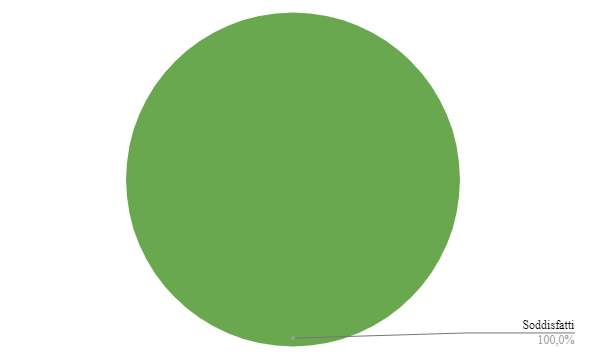
\includegraphics[width=1\textwidth]{../Images/SpecificaTecnica/req_obbligatori.PNG}
    \caption{Requisiti obbligatori soddisfatti}
    \label{fig: reqob}
\end{figure}

\end{document}
